\section{Dominant Background: Standard Model $t\tbar$}
\label{sec:Bkg:ttbar}

\indent The dominant background in this analysis is SM $\ttbar$.  After signal selection $\ttbar$ still accounts for $60-80$\% of the background depending on $\RISR$ range.  This section covers in detail the properties and treatment of SM $\ttbar$ in this analysis.  The section \ref{sec:Bkg:ttbar:Pop} demonstrates that there exist two kinematically distinct populations of SM $\ttbar$, each with unique characteristics and observables.  Section \ref{sec:Bkg:ttbar:CR} describes how we are able to directly measure the amount of $\ttbar$ in the signal region using a one-lepton control region.  \\

%Section \ref{sec:Bkg:ttbar:Sel} explores the kinematics of $\ttbar$ events after signal region selection.  

%\indent The $\met>250 \gev$ requirement selects $\ttbar$ with boosted leptonic tops because a top at rest cannot produce a neutrino with 250 $\gev of $\pt$.  After zero-lepton preselection, two kinematically distinct populations of $\ttbar$ exist.  One $\ttbar$ population use strong ISR to boost both tops. The other population uses boosts the leptonic top against the hadronic top in a back-to-back fashion. Section \ref{sec:Bkg:ttbar:Pop} describes these two kinematically distinct populations of $\ttbar$ in greater detail.   \\

%\indent Section \ref{sec:Bkg:ttbar:Sel} describes the signal selections used to remove the majority of $\ttbar$ background while retaining most of the signal.  These selection targets the larger and kinematically different population of $\ttbar$ that does not have strong initial state radiation.  $\ttbar$ with strong ISR appears more signal like and 90\% of all $\ttbar$ backgrounds after signal region selection are $\ttbar$ events with at least $400$ GeV of true initial state radiation.  These same selections are also very effective at removing subdominant SM backgrounds such as W+jets and Z+jets. \\

%\indent Section \ref{sec:Bkg:ttbar:CR} describes how we are able to directly measure the amount of $\ttbar$ background that is produced with strong initial state radiation in data using an one-lepton control region.  We avoid relying on theory predictions on the amount of ISR $\ttbar$ is expected to produce.  In this way, the control region allows us to minimize the amount of systematic uncertainties in the SR. \\

\subsection{Two Kinematically Distinct Populations of $t\tbar$}
\label{sec:Bkg:ttbar:Pop}

%define single hadronic tau

\indent The $\ttbar$ production and decay is shown in Figure \ref{fig:ttbar:feynDiag}.  Each top decays to a $W$ boson and $b$ quark and then in turn the W can decay into two quarks or a lepton and a neutrino. Depending on the number of leptons produced in the two $W$ boson decays, the $\ttbar$ decay channels are referred to as the zero-lepton, the single-lepton, or the dilepton channels.  The zero-lepton decay channel is also called the all-hadronic decay channel because all $\ttbar$ decay products are quarks in this channel.  \\

\indent The decay channels that produce leptons are further categorized by the type of lepton produced.  For example, the single tau $\ttbar$ decay channel has one $W$ that decays leptonically to a tau and a neutrino and the second W decays hadronically into two quarks.  The single muon decay channel has one $W$ that decays leptonically to a muon and a neutrino and the second W decays hadronically into two quarks.  \\

\begin{figure}[h!]
  \centering
	\includegraphics[width=0.65\textwidth]{./figures/feynDiag/ttbar_decay.jpg}
%	\caption[The $\ttbar$ production and decay Feynman diagram.]{ The $\ttbar$ production and decay Feynman diagram.  Each top decays to a $W$ boson and $b$ quark and then the W decay in turn to two quarks or a lepton and a neutrino. $\ttbar$ decay channels are classified according to the number and type of leptons produced. The different decay channels are referred to as the zero-lepton, the single-lepton, or the dilepton channels. The zero-lepton decay channel is also called the all-hadronic decay channel because all $\ttbar$ decay products are quarks in this channel.  Decay channels that also produce leptons are further separated by the type of lepton produced.  For example, the single tau $\ttbar$ decay channel has one $W$ that decays leptonically to a tau and a neutrino and the second W decays hadronically into two quarks. }
\caption[The $\ttbar$ production and decay Feynman diagram.]{ The Feynman diagram for the $ pp \rightarrow \ttbar \rightarrow W^{+}b + W^{-}\bar{b} \rightarrow ffb+ffb$ process.  The $\ttbar$ decay channels are classified according to the number and type of leptons produced. The different decay channels are referred to as the zero-lepton, the single-lepton, or the dilepton channels. The zero-lepton decay channel is also called the all-hadronic decay channel because all $\ttbar$ decay products are quarks.  Decay channels that also produce leptons are further separated by the types of lepton produced.  For example, the single tau $\ttbar$ decay channel has one $W$ that decays leptonically to a tau and a neutrino and the second W decays hadronically into two quarks. }
\label{fig:ttbar:feynDiag}
\end{figure}

\indent After the zero-lepton preselection, $\sim80$\% of $\ttbar$ events decay via the single tau channel.  $\sim15$\% of $\ttbar$ events decay via the single electron or single muon channels.  The electron and muon either doesn't pass the $\pt$ selection or the lepton is removed because it is too close to another jet or is misreconstructed as a jet. The final $\sim5$\% are due to dileptonic decays. Fully hadronic $\ttbar$ is negligible after signal region selections because fully hadronic $\ttbar$ produces little intrinsic $\met$. \\

\indent  The $\met>250 \gev$ requirement in preselection selects for $\ttbar$ with a boosted leptonic top.  A top at rest simply does not have enough energy to produce a neutrino with 250 $\gev$ of $\pt$. The leptonic top can gain boost mainly through one of two ways.  Either the leptonic top recoils in a back-to-back fashion against the hadronic top or both tops can recoil against strong ISR.  \\

%\indent Most $\ttbar$ events has one top that decays leptonically and the other top decaying fully hadronically after zero-lepton preselection. The leptonic top also produces a neutrino that satisfies the $250$ GeV of \MET requirement.  In most cases, the lepton is a tau that decays hadronically and registers as jet in calorimeter instead of a lepton.  In a smaller fraction of events a muon or electron is produced but the lepton is lost because of a number of reasons.  For example, the lepton can have too low $\pt$ to be reconstructed, or can be removed because they were to close to another jet or an electron is misreconstructed as a jet.  \\

%\indent Regardless of the exact decay channel, a top decaying at rest cannot generate enough momenta for the neutrino to have $250$ GeV of pt.  The top decaying via a tau or lepton, called the leptonic top, must therefore be boosted to have a high probability of satisfying the $250$ GeV \MET requirement.  The leptonic top can gain this boost through one of two ways.  Either the leptonic top recoils in a back-to-back fashion against the hadronic top or both tops recoil against strong ISR.  \\

\indent In both situations the thrust axis, the axis of maximum back-to-back $\pt$, contains important information.  In the case where the leptonic top is recoiling against the hadronic top, the thrust axis lines up along the two tops' axis of back-to-back boost.  In the case where both tops are boosted by strong ISR, the thrust axis approximates the $\ttbar$ and ISR axis of back-to-back recoil. An artistic representation of the role of the thrust axis in each $\ttbar$ population can be seen in Figure \ref{fig:ttbar:2pop}. \\

\begin{figure}[h!]
  \centering
	\includegraphics[width=0.65\textwidth]{./figures/strategy/ttbar_2pop.png}
	\caption[Schematic depiction of the $\ttbar$ two tops back-to-back population and the $\ttbar$+hard ISR population after the zero-lepton preselection.]{Schematic depiction of the $\ttbar$ back-to-back $\ttbar$ population and the $\ttbar$+hard ISR population after the zero-lepton preselection. The two example events' thrust axes are aligned.  The hemisphere containing $\met$ has significantly higher jet multiplicities and total energy in $\ttbar$+hard ISR events. }
\label{fig:ttbar:2pop}
\end{figure}

\indent Only the leptonic top is boosted towards the same hemisphere as the $\met$ when the top and anti-top are back-to-back to one another.  In comparison, both tops are boosted towards the hemisphere containing $\met$ in the $\ttbar$ with strong ISR. Therefore the $\ttbar$+hard ISR population has a much higher jet multiplicity and total energy in the $\met$ hemisphere.  Hence, we can use observables such as $\NjV$ and $\MS$ to distinguish $\ttbar$ plus large ISR events from $\ttbar$ back-to-back recoil events.   \\

%\subsection{Properties of SM $t\tbar$ in Signal Region}
%\label{sec:Bkg:ttbar:SR}

%\indent Stop signal is expected to have a higher jet multiplicities and energy in the hemisphere containing $\met$ then both $\ttbar$ populations.  The stringent signal region requirements on the jet multiplicities and total energy of the sparticle hemisphere effectively eliminate the $\ttbar$ back-to-back $\ttbar$ population and also rejects approximately $2/3$ of $\ttbar$+hard ISR population.  A detailed explanation of signal region design and performance can be found in chapter \ref{chap:SignalRegion}. \\

%\indent The $\ttbar$ events that survives the signal region selections are composed of almost exclusively $\ttbar$ that are also produced with strong ISR.  Approximately 90\% of the $\ttbar$ events in signal region have an ISR $\pt$ of at least 400 $\gev$.  The distribution of true ISR $\pt$ for $\ttbar$ that survive the signal selections can be seen in Figure \ref{fig:ttbar:SR:trueISRpt}.\\

%\begin{figure}[h!]
%  \centering
%	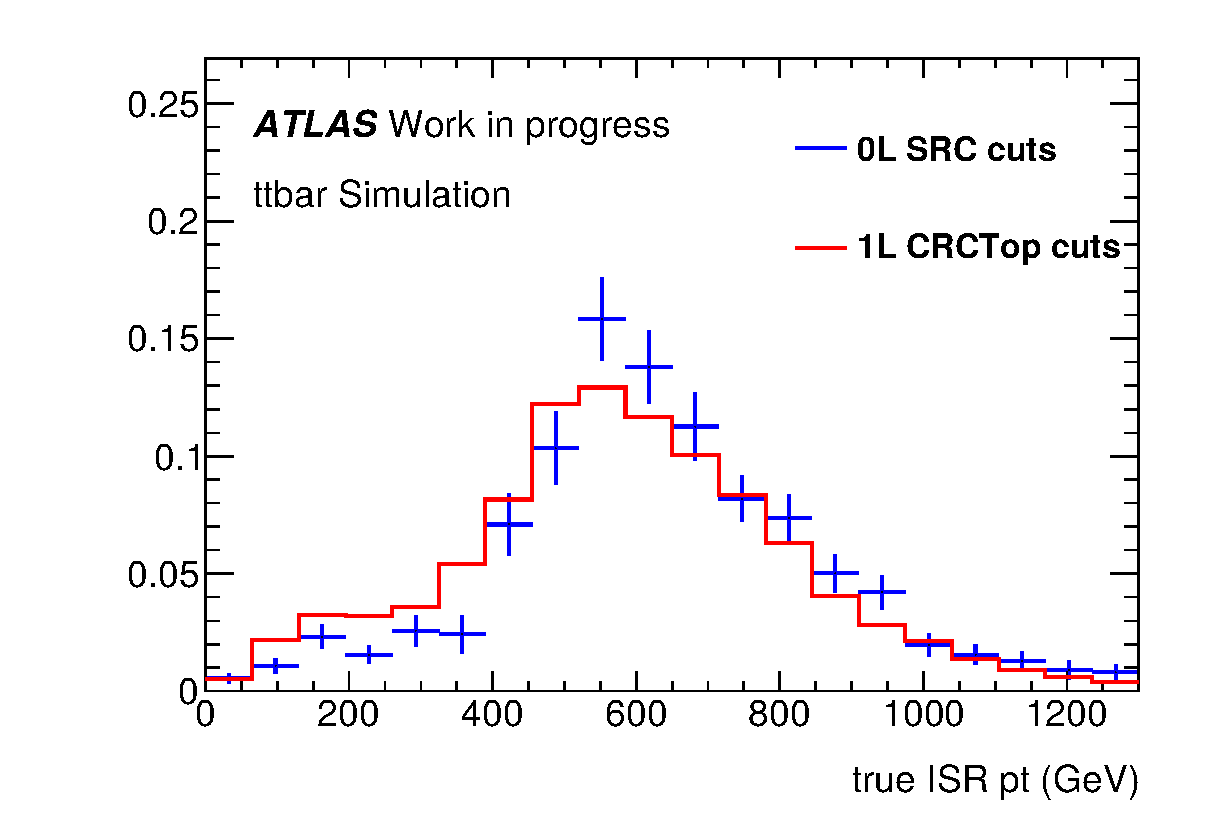
\includegraphics[width=0.65\textwidth]{./figures/ttbar/truePtISR_SRC_CRC_compare.eps}
%\caption{\label{fig:ttbar:CR:trueISRpt}{Distribution of true ISR $\pt$ for $\ttbar$ that survive the signal selections}}
%\end{figure}

%\indent In terms of branching fractions, the majority of $\ttbar$ branching fractions are to hadronic taus.  80\% of the $\ttbar$ has one top decay via a single hadronic tau and the other top decays fully hadronically.  $15$\% of the $\ttbar$ events decay via the single lepton channel where the lepton is an electron or a muon.  The lepton becomes lost because either it has too low $\pt$ to be reconstructed, removed because they were to close to another jet or is misreconstructed as a jet. The rest of the five\% composed of di-leptonic or lepton and tau $\ttbar$ events. Essentially no fully hadronic $\ttbar$ survives the zero-lepton selection because fully hadronic $\ttbar$ do not make any hard neutrinos directly from the top decay.  \\
%\indent With such a large fraction of background coming from taus one might suspect setting up some sort of tau rejection.  However we found that a rejection based on loose tau IDs did not improve sensitivity.  The loss of signal was too large to justify the improvement in signal to background ratio.  The high jet multiplicity in signal gives a high probability of false positives.
%\indent Accepting mainly $\ttbar$ decay to hadronic taus gives a large boost signal to background due to branching fractions alone.  The two tops in signal events decay mainly through the fully hadronic channel.  Fully hadronic decays account for 44\% of all $\ttbar$ decays.  On the other hand, the $\ttbar$ background mainly decay via hadronic taus which only accounts for about 10 of all $\ttbar$ decays.  We therefore gain a factor of 5 in signal to background ratio just by working in the zero-lepton channel. This not only gains us a great boost in sensitivity in our SR.  It also allows us to design a $\ttbar$ control region with very similar selections to the signal region but just in the single lepton channel.  We can avoid high signal contamination in our control region because both signal and background are mainly coming from single lepton decays in the one-lepton channel.  As such, we no longer gain this factor of 5 in S/B based on branching fraction in the control region.  The details of the $\ttbar$ control region is described in section \ref{sec:Bkg:ttbar:CR} \\  

\subsection{Predicting the amount of $\ttbar$ in Signal Region using a One-Lepton Control Region}
\label{sec:Bkg:ttbar:CR}

\indent The stop signal is expected to have higher jet multiplicities and total energy in the hemisphere containing $\met$ than both $\ttbar$ populations.  The stringent signal region requirements on the jet multiplicities and total energy of the sparticle hemisphere effectively eliminate the $\ttbar$ back-to-back $\ttbar$ population and also reject approximately $2/3$ of the $\ttbar$ plus large ISR population.  A detailed explanation of the signal region design and performance can be found in chapter \ref{chap:SignalRegion}. \\

%The $\ttbar$ events that survives the signal selections are composed of almost exclusively $\ttbar$ that are also produced with large ISR.  
\indent Approximately 90\% of the $\ttbar$ events in the signal region have at least 400 $\gev$ of real ISR $\pt$.  A back of the envelope calculation shows that we need around 550-600 $\gev$ of ISR $\pt$ to boost the $\ttbar$ neutrino to above 250 $\gev$ of $\pt$.  The neutrino must share the total $\ttbar$ $\pt$ with the five other $\ttbar$ decay products and is not particularly efficient at absorbing ISR $\pt$.  \\

\indent Figure \ref{fig:ttbar:SR:trueISRpt_presel_SRC1} shows that the true ISR $\pt$ distribution for $\ttbar$ in the signal region peaks at approximately 550 $\gev$.  In comparison, the true ISR $\pt$ distribution after preselection peaks at zero and rapidly falls with increasing ISR $\pt$.  This demonstrates that the additional signal region requirements select mainly for $\ttbar$ with high ISR $\pt$.  \\

\begin{figure}[h!]
  \centering
	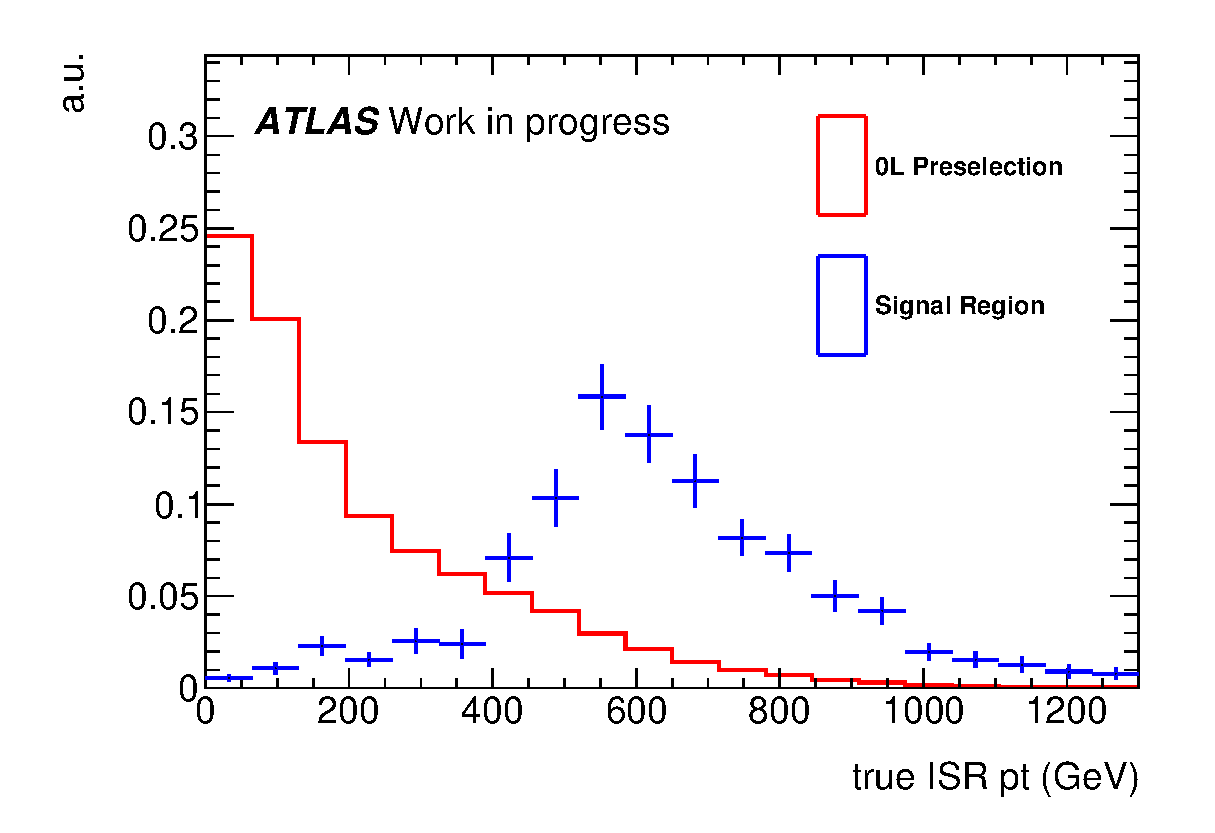
\includegraphics[width=0.80\textwidth]{./figures/strategy/Compare0L_truth.eps}
\caption[Distribution of true ISR $\pt$ for $\ttbar$after the zero-lepton preselection and after all signal region selections]{Distribution of true ISR $\pt$ for $\ttbar$ after the zero-lepton preselection and after all signal region selections.  Both distributions have been normalized to unit area.}
\label{fig:ttbar:SR:trueISRpt_presel_SRC1}
\end{figure}

\indent A direct consequence of selecting for only high ISR $\ttbar$ events is that the predicted $\ttbar$ background rates in the signal region are directly related to the amount of ISR/FSR in the MC.  The next-to-leading order (NLO) \textsc{Powheg+\pythia6} $\ttbar$ MC has a $\sim30$\% ISR/FSR systematic uncertainty in the signal region.  The ISR/FSR uncertainty would dominate the systematic uncertainty in this analysis if we relied on MC alone to predict the $\ttbar$ background in the signal region.  \\

\indent In order to decrease the ISR/FSR uncertainty, we directly measure the $\ttbar$+hard ISR rate in data using a one-lepton $\ttbar$ control region (CRTopC).  The lepton refers only to an electron or muon in this context because they can be reconstructed with much greater purity than taus.  The control region CRTopC selections are defined in Table \ref{tab:ttbar1LepCRISR_def}. All variables used are defined in section \ref{Jigsaw:Variables}. \\

\begin{table}[h!] 
 \caption{One-lepton $\ttbar$ control region (CRTopC) definitions. The one-lepton preselections defined in Table~\ref{tab:1Lcommon} are also applied. }
  \label{tab:ttbar1LepCRISR_def}
  \begin{center}
    \def\arraystretch{1.4}%
    \begin{tabular}{c|c} \hline\hline
      {\bf Variable}     & 1 lepton $\ttbar$ control region \\ \hline \hline
      \multicolumn{2}{c}{1 Lepton Preselection}  \\ \hline
      $N_{lep}$  & 1                   \\
      \mtlepmet          & $<80\gev$           \\ 
      \mindrblep         & $<2.0$              \\ 
      \NjV               & $\ge5$              \\
      \NbV               & $\ge1$              \\
      \pTSFour           & $>40\gev$           \\
      \PTISR             & $\ge 400$           \\ \hline \hline
    \end{tabular}
    \end{center}
\end{table}%

\indent In the one-lepton control region, the lepton is included as a ``jet'' in the Jigsaw ISR algorithm and will be counted as a sparticle jet or an ISR jet depending on which hemisphere it falls in.  The lepton is meant to play the role of a hadronic tau jet in the zero-lepton signal region.  This approximation is justified since $\sim80$\% of all $\ttbar$ events in the signal region decay via the hadronic tau channel.  \\

\indent The control region CRTopC uses similar selections on the same kinematic variables as the signal region.  In this way, the control region CRTopC captures the same kinematic features as the signal region by also targeting $\ttbar$ with high ISR $\pt$. Some signal region requirements such as the correlations on ISR and $\met$ are removed to increase statistics and lower signal contamination.  For example, the signal region $\dphiISRI > 3.0$ requirement is removed.  The $\dphiISRI$ variable specifies the direction of neutrino relative to the direction of the ISR.  A requirement of $\dphiISRI>3.0$ essentially selects specific alignments between the $\ttbar$ decay axis and the $\ttbar$ vs ISR boost axis.  Removing this requirement opens up more phase space for $\ttbar$ to decay but does not change the requirement on high ISR $\pt$. \\

\indent The $\pTjV>50\gev$ requirement is relaxed to $\pTjV>40\gev$ in order to increase statistics in the CR.  The $\pTjV$ requirement specifies the $\pt$ of the 4th jet in the sparticle system.  The $\pTjV$ variable is correlated with amount of ISR/FSR in the MC because there is a chance that the 4th most energetic jet in the sparticle system is from radiation and not from a top decay.  However it is more important to accurately gauge the amount of hard ISR of order hundred or more GeV that boosts the entire $\ttbar$ system than the amount of additional radiation in the same hemisphere as $\ttbar$. We found that loosening the $\pTjV$ requirement to 40 GeV does not result in a large difference between the control and signal regions' true ISR $\pt$ distributions . \\

%If stop mass is significantly larger than $m_{\ninoone}+m_t$ then the stop decays tend to produce more $\met$. 
\indent   A $\mtlepmet$ less than $80\gev$ requirement selects events with a transverse mass that is consistent with a W boson.  The $\mtlepmet$ increases $\ttbar$ purity and removes signal contamination.   A $\mindrblep$ less than $2.0$ requirement is also added to increase $\ttbar$ purity and ensure orthogonality to the $W$+jets control region. $\mtlepmet$ is defined in equation \ref{eqn:mtlep} and $\mindrblep$ is defined in equation \ref{eqn:mindrblep}. \\

\begin{equation}
\mtlepmet = (E_{T}^{lep}+\met)^{2}-({\vec {p}}_{T}^{lep}+{\vec {E}}_{T}^{miss})^{2} =m_{lep}^{2}+2(E_{T}^{lep}\met-{\vec {p}}_{T}^{lep}\cdot {\vec {E}}_{T}^{miss})
\label{eqn:mtlep}
\end{equation}

\begin{equation}
\mindrblep = \min_{jets~with~two~highest~b-tagging~values} \sqrt{ \Delta\eta(bjet, lep)^2 + \Delta\phi(bjet, lep)^2}
\label{eqn:mindrblep}
\end{equation}


\indent Figure \ref{fig:ttbar:CR:trueISRpt} shows the true ISR $\pt$ distribution for $\ttbar$ in the control region and the signal region.  Both distributions peak at roughly 550 $\gev$ and have similar shapes.  We use the one-lepton control region to measures the amount of $\ttbar$ plus high ISR $\pt$ events using data.  By normalizing $\ttbar$ background rates to the control region, we are able to limit the ISR/FSR uncertainty to below 10\% for all $\RISR$ regions.  \\

\indent The similar kinematic selection between the control region CRTopC and the signal region cancels many systematic uncertainties.   For example, the 6\% uncertainty on jet energy resolution is partial due to the similar jet $\pt$ requirements between the control region and the signal region. A more detailed discussion of systematics can be found in chapter \ref{chap:Uncertainties} \\

%a.u. on the plot
\begin{figure}[h!]
  \centering
	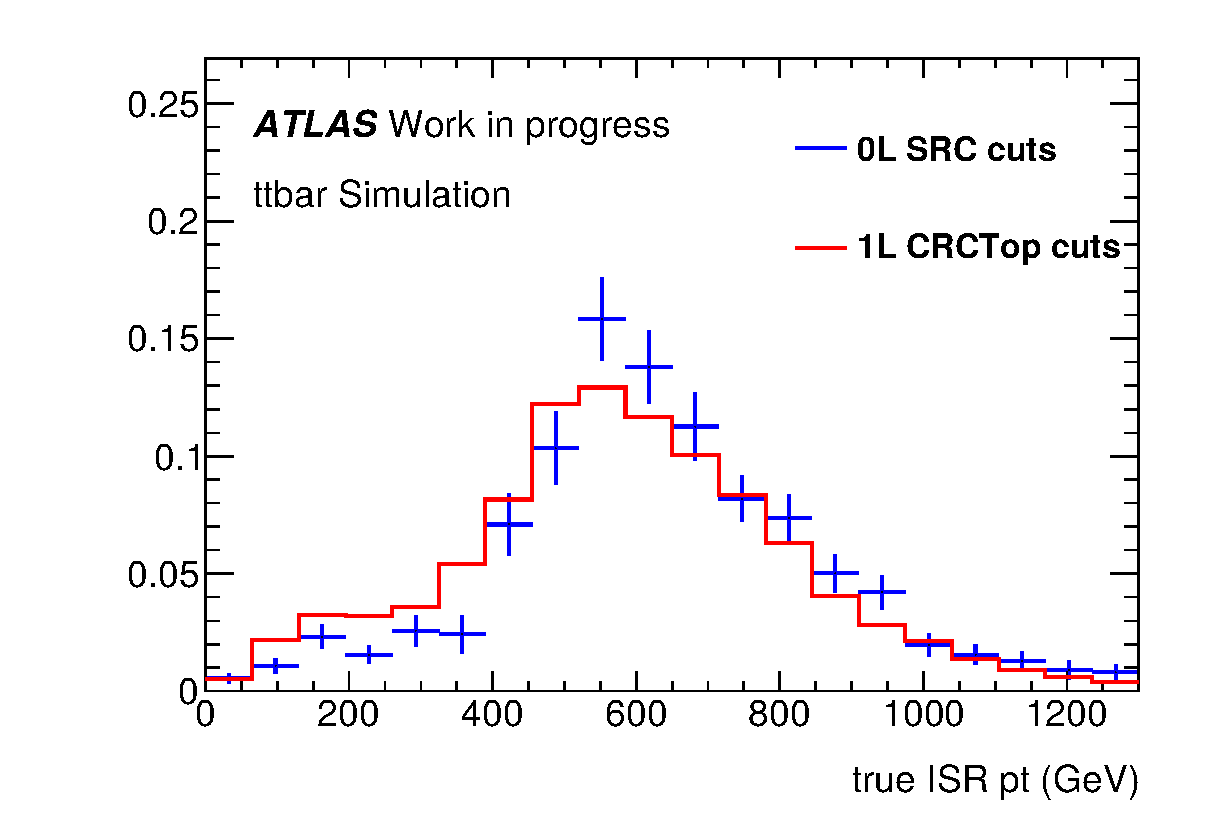
\includegraphics[width=0.65\textwidth]{./figures/ttbar/truePtISR_SRC_CRC_compare.eps}
	\caption[The true ISR $\pt$ distribution for $\ttbar$ events after signal region and $\ttbar$ control region (CRTopC) selections]{The true ISR $\pt$ distribution for $\ttbar$ events after signal region and $\ttbar$ control region (CRTopC) selections.  Both control and signal region distributions peak at roughly 550 $\gev$ demonstrating that the one-lepton control region and the zero-lepton signal region select for the same $\ttbar$+hard ISR events.  Therefore, the one-lepton control region is able to directly measure the amount of $\ttbar$ with high ISR $\pt$ directly from data.  This lets us predict the $\ttbar$ background rate in the signal region with minimal extrapolation between the control region and the signal region.}
	\label{fig:ttbar:CR:trueISRpt}
\end{figure}

\subsubsection{Control Region CRTopC Signal Contamination}

\indent The control regions are designed to have low expected signal rates.  If stop events are present in the control region then they can be misinterpreted as additional SM background.  In this way, a high expected signal rate in the control region decreases signal sensitivity.  The fractional signal contamination can be quantified as the signal over background (S/B) ratio in the control region. \\% In general signal contamination should not exceed $\sim10$\% in any control region.\\

\indent Signal contamination in the control region CRTopC ranges from 1\% at high stop masses to 12\% at low stop masses for all stop masses that we are sensitive to and are not already excluded by previous stop experiments. \\% Signal contamination from stop masses that the analysis is not sensitive to are not important.  If the stop exists but has a mass that the analysis is not sensitive to, the stop will not be discovered regardless of the amount of signal contamination in the control region.\\

\indent The largest signal contamination occurs at a stop mass of 225 to 250 $\gev$.   Here, the signal contamination approaches 12\% due to the large stop production cross section.  Lower stop masses result in higher signal contamination but our search does not have sensitivity to regions below 225 $\gev$.  \\

\indent The fact that the control region CRTopC can attain such low signal contamination while selecting for $\ttbar$ background with similar kinematic features to the signal region is impressive.  The signal region has a S/B ratio of approximately 2$\:$1 for stop masses between 250 $\gev$ and 400 $\gev$.   In comparison, the control region CRTopC is able to achieve the fractional signal contamination of around 5 to 12\% for the same stop masses.  \\

\indent The control region CRCTop has a factor of 20-40 lower S/B ratio when compared to the signal region because of mainly two reasons.  First, the CRCTop is a one-lepton region while the signal region is a zero-lepton region. \\

\indent The signal region primarily selects for stops that decay fully hadronically with a $\sim44$\% branching fraction.  However, the $\ttbar$ background in the signal region mainly decays via the single hadronic tau decay channel with only a 10\% decay fraction.  The signal region therefore gains a factor of 5 in S/B ratio because of the difference in stop and $\ttbar$ branching fractions.    \\

\indent Meanwhile, the one-lepton control region primarily selects events that decay via the single muon and single electron decay channels in both stop signal and $\ttbar$ background.  Signal and background therefore has similar decay fractions in the control region CRTopC.  This means the control region CRTopC has a factor of 5 less S/B ratio than the signal region simply because of branching fractions.  \\

\indent The signal region also gains in S/B ratio by requiring strong correlations between the ISR system and $\met$.  The signal region separates the signal and background into 5 bins in $\RISR$.  This targets the signal's peak in $\RISR$.  In contrast, the control region CRTopC does not have separate $\RISR$ bins.  Integrating over all $\RISR$ instead of specifically targeting the bins under the signal region peak decreases the S/B ratio by a factor of 2-5 depending on the stop mass and location of the signal $\RISR$ peak.  \\

\indent At the same time, removing the $\dphiISRI > 3.0$ requirement in the control region decreases the S/B ratio by another factor of 3.  Removing the requirements on the ISR and $\met$ correlations open up more phase space but do not change the requirement on strong $\ttbar$ ISR $\pt$.  \\

\indent These factors combine to make up the factor of $\sim40$ decrease in the S/B ratio between the signal region and the control region CRTopC; all the while preserving the agreement in the true $\ttbar$ ISR $\pt$ distribution shown in Figure \ref{fig:ttbar:CR:trueISRpt}. \\

\subsubsection{$\ttbar$ Control Region Yields and Distributions}

\indent Distribution of important variables after a background-only fit to $\intlumi$ $\ifb$ of data are shown for the control region CRTopC in Figure \ref{fig:CRTopC1} and \ref{fig:CRTopC2}.   There is a noticeable trend in the data over MC comparison in the CRTopC $\pTISR$ distribution.  The disagreement is not surprising given that a priori we have a 30\% uncertainty due to the ISR/FSR uncertainty.  This further demonstrates the need for a control region that directly measures the amount of $\ttbar$ with strong ISR using data. \\

\indent The fitted normalization scale factor for $\ttbar$ is 0.707. This scale factor is quiet different from 1.0 which indicates that the $\ttbar$ MC does a poor job of modeling the high ISR $\pt$ phase space.  Again, this difference is not unexpected given the 30\% ISR/FSR uncertainty on $\ttbar$ MC in this high ISR $\pt$ region.  \\

\begin{figure}[h!]
  \begin{center}
      \begin{subfigure}[b]{0.40\textwidth}    
    	 \includegraphics[width=\textwidth]{figures/plotRegion/Met_CRTopC_log.eps}
                \caption{ }
    \end{subfigure}
        \begin{subfigure}[b]{0.40\textwidth}    
    	 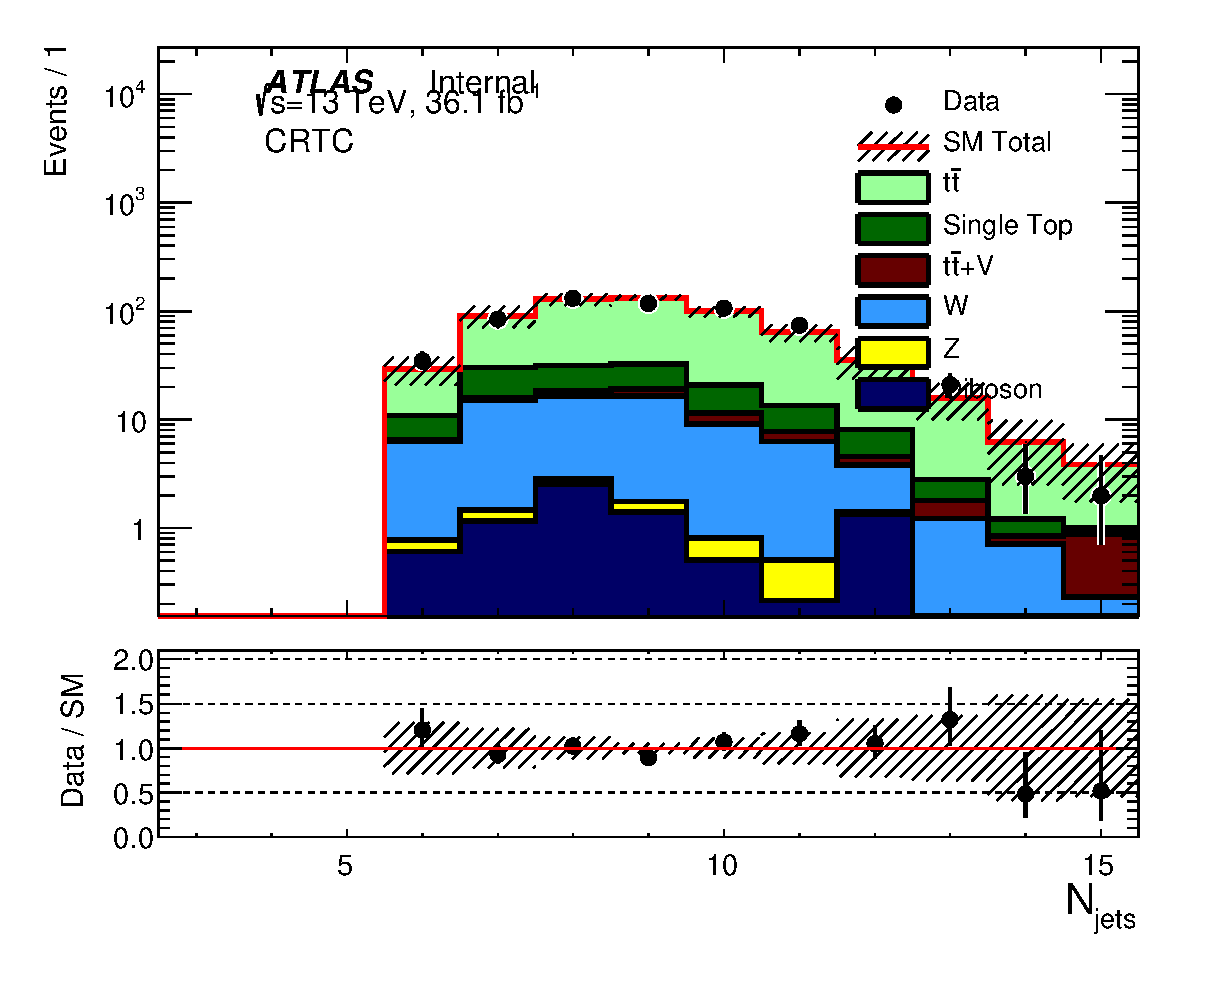
\includegraphics[width=\textwidth]{figures/plotRegion/NJets_CRTopC_log.eps}
                \caption{ }
    \end{subfigure}
    \begin{subfigure}[b]{0.40\textwidth}    
    	 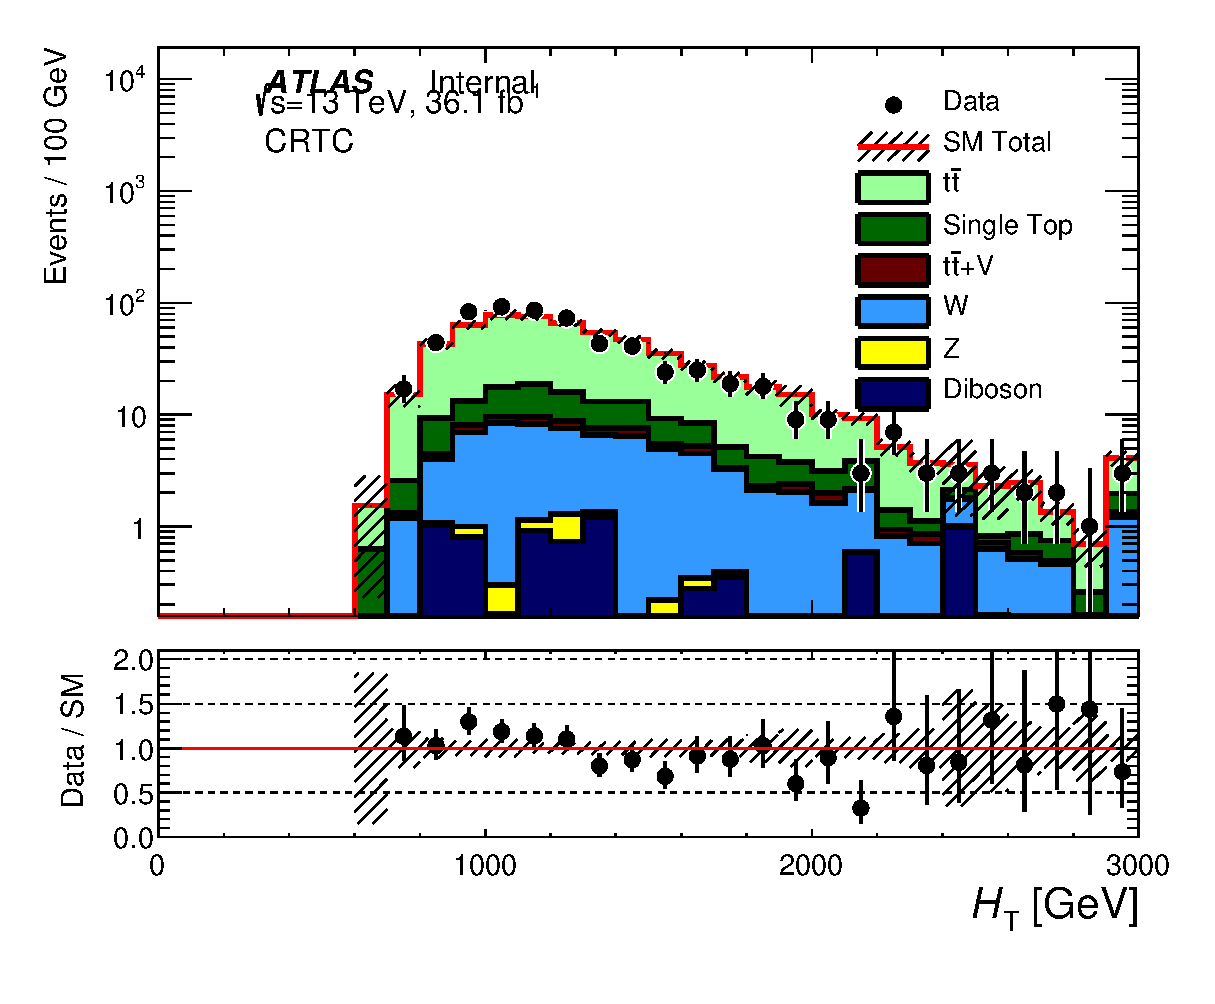
\includegraphics[width=\textwidth]{figures/plotRegion/Ht_CRTopC_log.eps}
                \caption{ }
    \end{subfigure}
    \begin{subfigure}[b]{0.40\textwidth}    
    	 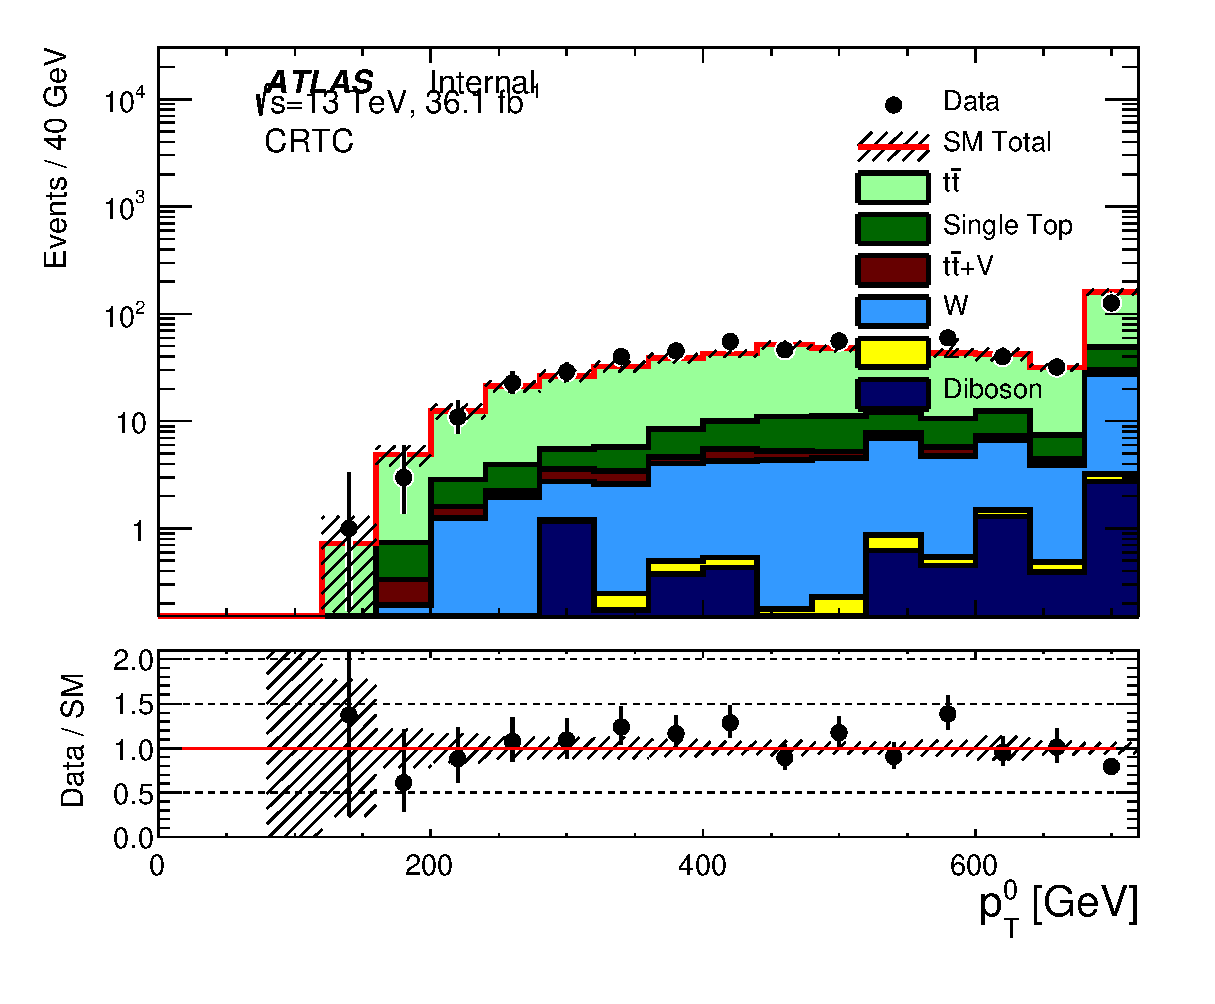
\includegraphics[width=\textwidth]{figures/plotRegion/JetPt_0__CRTopC_log.eps}
                \caption{ }
    \end{subfigure}
    \begin{subfigure}[b]{0.40\textwidth}    
    	 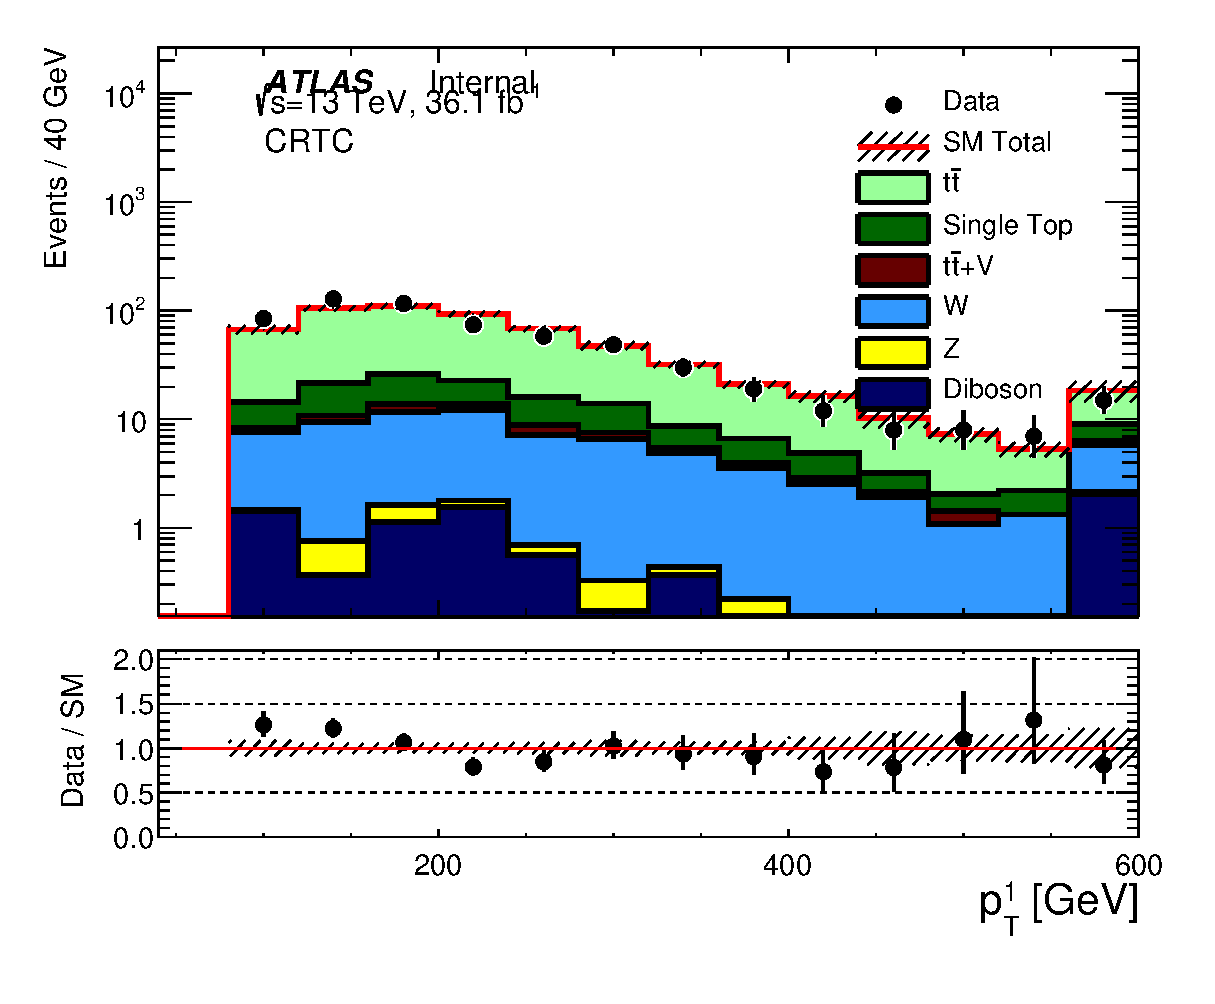
\includegraphics[width=\textwidth]{figures/plotRegion/JetPt_1__CRTopC_log.eps}
                \caption{ }
    \end{subfigure}
    \begin{subfigure}[b]{0.40\textwidth}    
    	 \includegraphics[width=\textwidth]{figures/plotRegion/JetPt_3__CRTopC_log.eps}
               \caption{ }
    \end{subfigure}
     \caption[One-lepton $\ttbar$ control region (CRCTop) distributions for $\intlumi$ $\ifb$ of data]{ One-lepton $\ttbar$ control region (CRCTop) distributions for $\intlumi$ $\ifb$ of data. The kinematic variables shown include (a) $\met$ (b) number of jets (c) $\HT$ (d) $\pt$ of the highest $\pt$ jet (e) $\pt$ of the 2nd highest $\pt$ jet (f) $\pt$ of the 4th highest $\pt$ jet. }% All backgrounds yields have been normalized to data by performing a background-only fit. The hashed area represents the uncertainty due to MC statistics and detector systematic uncertainties.}
     %One-lepton $\ttbar$ control region (CRCTop) distributions for $\intlumi$ $\ifb$ of data. The kinematic variables shown include (a) $\met$ (b) number of jets (c) $\HT$ (d) $\pt$ of the highest $\pt$ jet (e) $\pt$ of the 2nd highest $\pt$ jet (f) $\pt$ of the 4th highest $\pt$ jet.  All backgrounds yields have been normalized to data by performing a background-only fit.  The ratio between data and MC is shown in the bottom panel. The hashed area in both the top and lower panel represents the uncertainty due to MC statistics and detector systematic uncertainties. }
  \label{fig:CRTopC1}
    \end{center}
\end{figure}

\pagebreak

\begin{figure}[h!]
  \centering
        \begin{subfigure}[b]{0.40\textwidth}  
    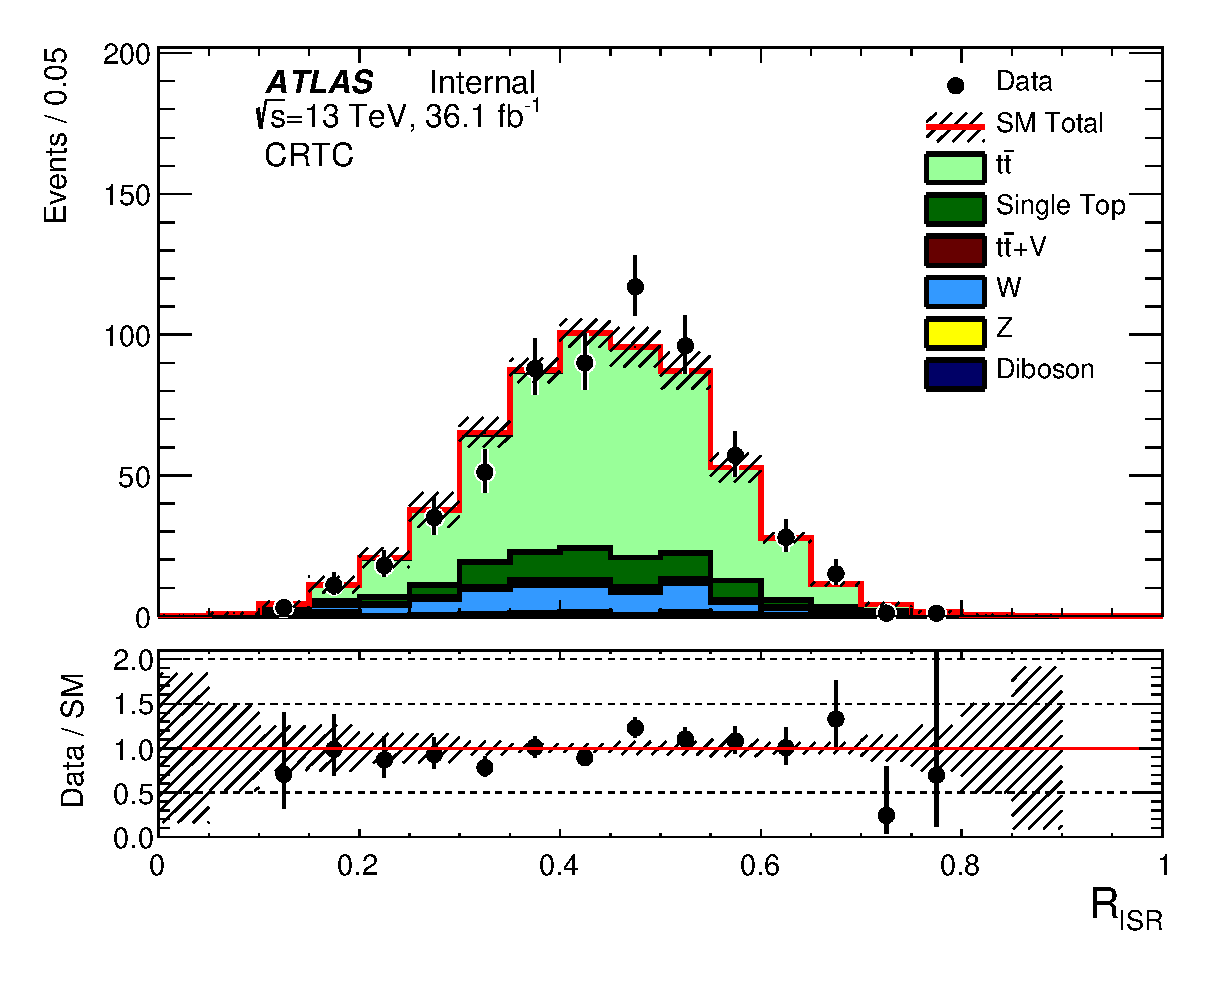
\includegraphics[width=\textwidth]{figures/ttbar/postfit/CA_RISR_CRTopC}
               \caption{ }
    \end{subfigure}
            \begin{subfigure}[b]{0.40\textwidth}  
    \includegraphics[width=\textwidth]{figures/ttbar/postfit/CA_pTISR_CRTopC}
               \caption{ }
    \end{subfigure}
            \begin{subfigure}[b]{0.40\textwidth}  
    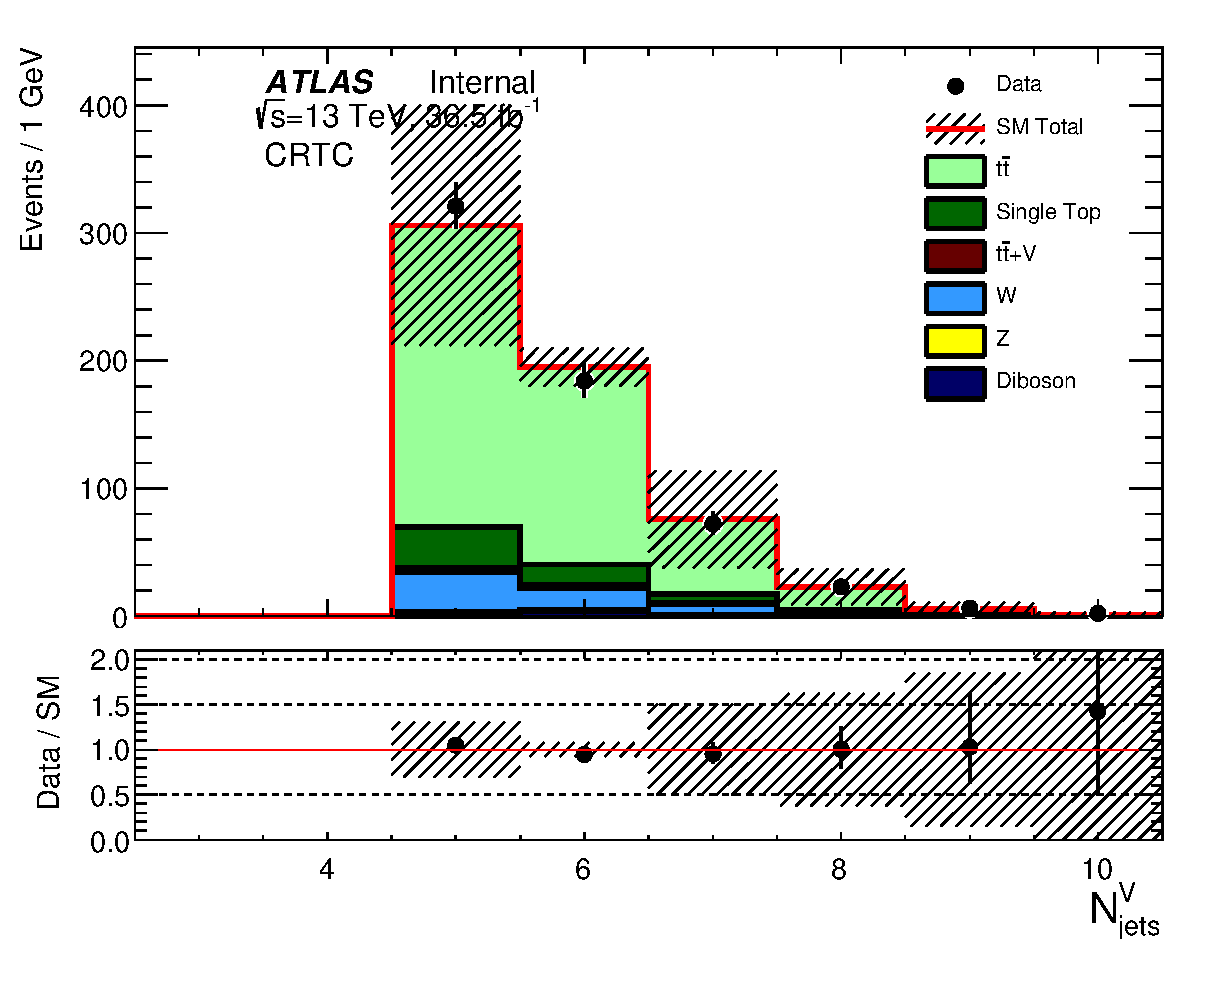
\includegraphics[width=\textwidth]{figures/ttbar/postfit/CA_NjV_CRTopC}
               \caption{ }
    \end{subfigure}
            \begin{subfigure}[b]{0.40\textwidth}  
    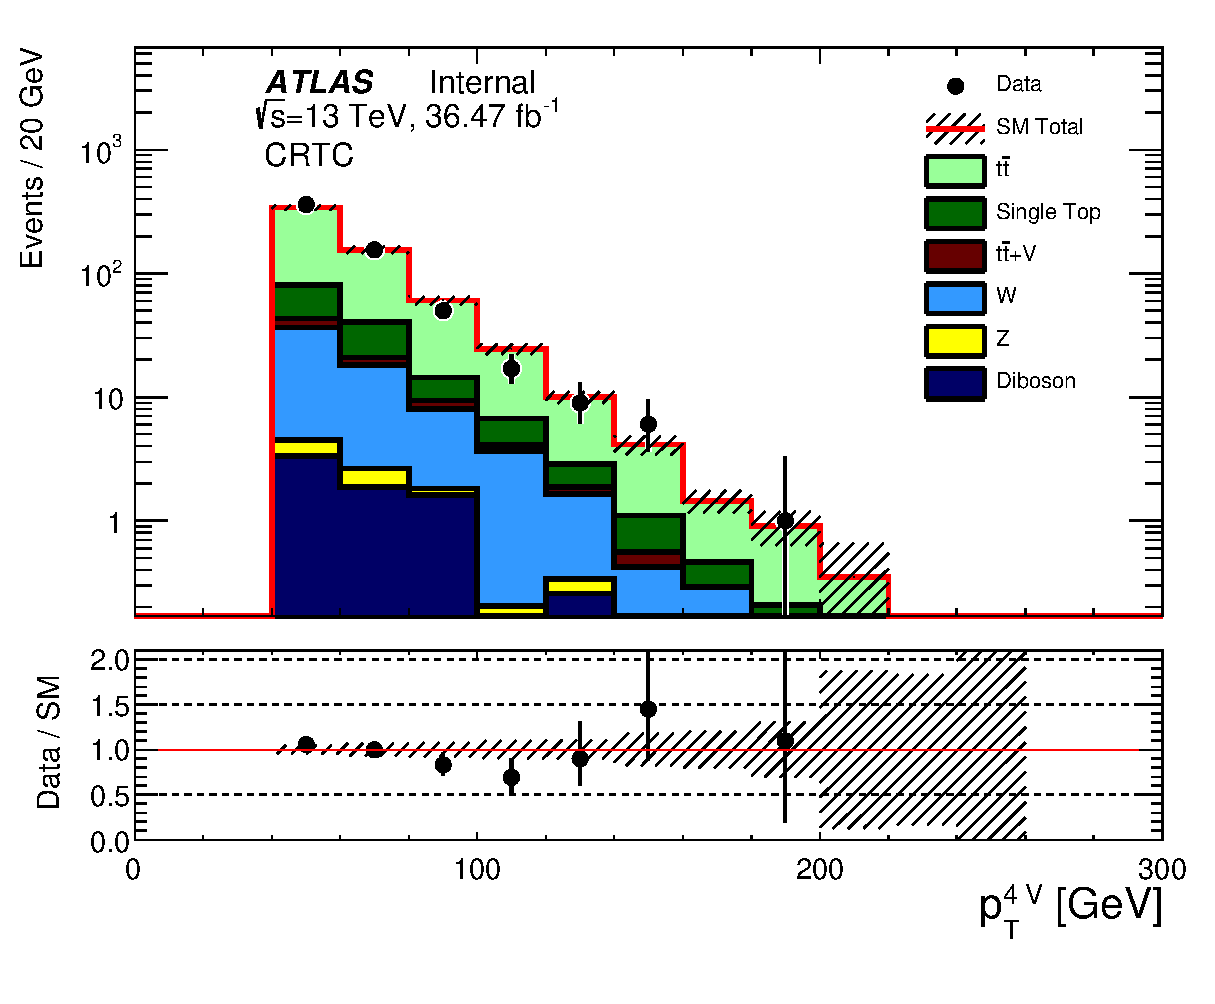
\includegraphics[width=\textwidth]{figures/ttbar/postfit/CA_pTjV4_CRTopC_log}
               \caption{ }
    \end{subfigure}
            \begin{subfigure}[b]{0.40\textwidth}  
    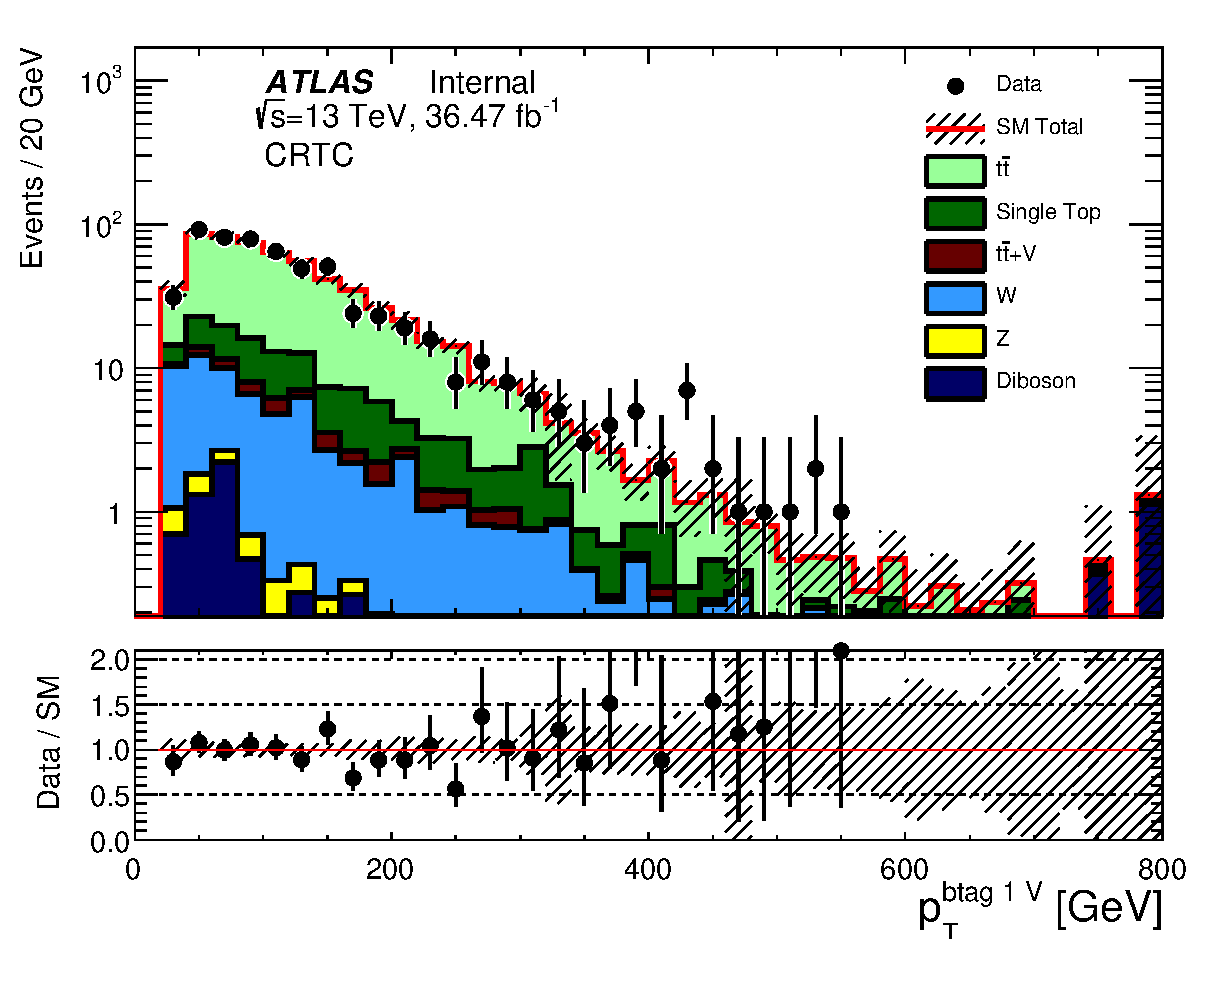
\includegraphics[width=\textwidth]{figures/ttbar/postfit/CA_pTbV1_CRTopC_log}
               \caption{ }
    \end{subfigure}
            \begin{subfigure}[b]{0.40\textwidth}  
    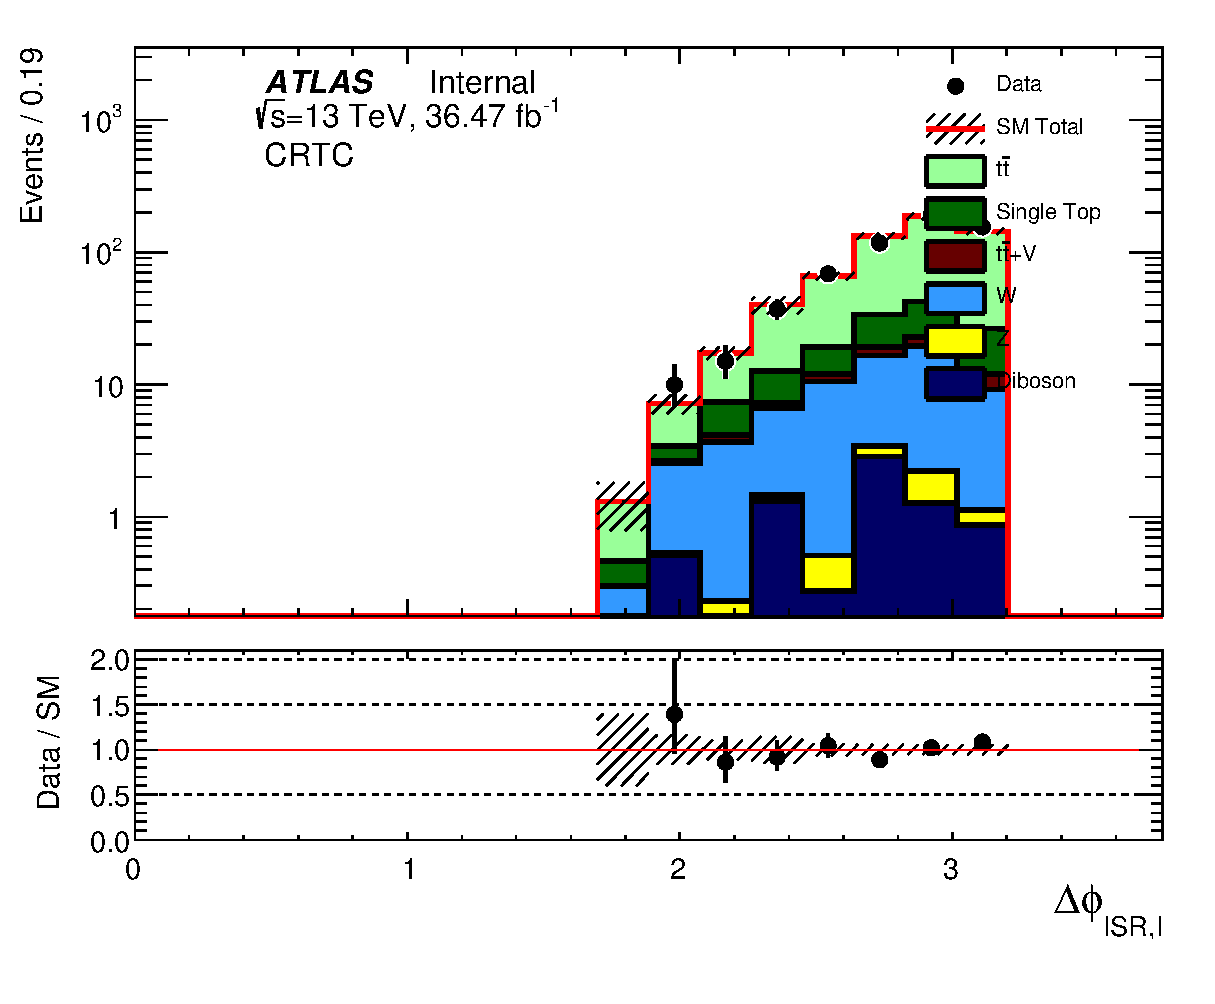
\includegraphics[width=\textwidth]{figures/ttbar/postfit/CA_dphiISRI_CRTopC_log}
               \caption{ }
    \end{subfigure}
       \caption[One-lepton $\ttbar$ control region (CRTopC) distributions for $\intlumi$ $\ifb$ of data]{One-lepton $\ttbar$ control region (CRCTop) distributions for $\intlumi$ $\ifb$ of data.  The kinematic variables shown include (a) $\RISR$ (b) $\PTISR$ (c) $\NjV$ (d) $\pTjV$ (e) $\pTbV$ (f) $\dphiISRI$.  } %All backgrounds yields have been normalized to data by performing a background-only fit.  The ratio between data and MC is shown in the bottom panel. The hashed area in both the top and lower panel represents the uncertainty due to MC statistics and detector systematic uncertainties.}
  \label{fig:CRTopC2}
\end{figure}

\indent There seems to be no significant slope in the data over MC comparison in the CRCTop $\pTjV$ distribution.  This is further evidence that the extrapolation from 40 to 50 GeV across $\pTjV$ is allowed.  No strong trends outside of statistical and systematic uncertainties are observed for any other distributions. \\

\indent The control region CRTopC yields from before and after the background-only fit can be found in Table \ref{table.bkgonly.CRTopC}.\\



\begin{table}[h!]
\begin{center}
\setlength{\tabcolsep}{0.0pc}
{\small
%%
\begin{tabular*}{\textwidth}{@{\extracolsep{\fill}}lr}
\noalign{\smallskip}\hline\noalign{\smallskip}
{\bf Yields}           & CRTopC                  \\[-0.05cm]
\noalign{\smallskip}\hline\noalign{\smallskip}
%%
Observed data events          & $611$                       \\
\noalign{\smallskip}\hline\noalign{\smallskip}
%%
Fitted SM bkg events         & $610.96 \pm 24.72$                     \\
\noalign{\smallskip}\hline\noalign{\smallskip}
%%
        Fitted $\ttbar$ events         & $461.47 \pm 31.85$                 \\
%%
        Fitted Wjets events         & $64.94 \pm 12.12$                    \\
%%
        Fitted Zjets events         & $2.15 \pm 0.90$                \\
%%
        Fitted TtbarV events         & $11.32 \pm 2.19$                    \\
%%
        Fitted SingleTop events         & $63.49 \pm 20.36$                   \\
%%
        Fitted Diboson events         & $7.58 \pm 2.84$                       \\
%%
        Fitted Multijets events         & $0.00 \pm 0.00$                    \\
%%     
 \noalign{\smallskip}\hline\noalign{\smallskip}
%%
MC exp. SM events              & $777.01 \pm 14.91$                   \\
\noalign{\smallskip}\hline\noalign{\smallskip}
%%
        MC exp. $\ttbar$ events         & $652.93 \pm 7.35$                     \\
%%
        MC exp. Wjets events         & $51.34 \pm 6.02$                 \\
%%
        MC exp. Zjets events         & $1.84 \pm 0.58$                 \\
%%
        MC exp. TtbarV events         & $8.78 \pm 0.90$                      \\
%%
        MC exp. SingleTop events         & $54.53 \pm 5.03$                  \\
%%
        MC exp. Diboson events         & $7.58 \pm 2.87$                     \\
%%
        MC exp. Multijets events         & $0.00 \pm 0.00$                   \\
%%     \\
\noalign{\smallskip}\hline\noalign{\smallskip}
Fitted $\ttbar$ normalization scale factor & $0.707 \pm 0.050$ \\
\noalign{\smallskip}\hline\noalign{\smallskip}
\end{tabular*}
%%%
}
\caption[CRTopC MC Yield and background-only fit results for $\intlumi$ $\ifb$ of data]{CRTopC MC Yield and background-only fit results for $\intlumi$ $\ifb$ of data. MC exp. events are expected background rates directly from MC predictions.  Fitted background event rates are the expected background rates after normalizing the MC to data by simultaneously fitting all control regions using a background only fit.  The fitted $\ttbar$ normalization scale factor is equal to (Fitted $\ttbar$ events)/(MC exp. $\ttbar$ events). The quoted uncertainties include statistical and systematic uncertainties. }
\label{table.bkgonly.CRTopC}
\end{center}
\end{table}
%

\subsection{Validating $\ttbar$ Predictions in Signal Region using a Zero-Lepton Validation Region}
\label{sec:Bkg:ttbar:VR}

\indent We also define a zero-lepton $\ttbar$ validation region to validate the predicted background rates in the signal region.  The $\ttbar$ validation region (VRTopC) is kinematically similar but completely orthogonal to the signal region.  In addition, the validation region must have limited signal contamination and high $\ttbar$ purity. \\

\indent The $\dphiISRI > 3.0$ selection in the signal region is inverted in the validation region to limit signal contamination. In signal, the neutralinos and the ISR tend to be back-to-back in $\phi$.  The neutralinos gain most of their momenta by recoiling against ISR and the correlation is strong. \\

\indent In contrast, $\dphiISRI$ has a different physical interpretation in SM $\ttbar$ events.   In $\ttbar$ events, $\dphiISRI$ specifies the neutrino direction relative to the direction of the ISR.  Inverting the $\dphiISRI$ selection selects for $\ttbar$ events with a different decay axis relative to $\ttbar$ vs ISR boost axis but does not change the requirements on strong ISR $\pt$.  \\

\indent For this reason, the $\dphiISRI < 3.0$ requirement in the validation region rejects $\sim50$\% of signal events while retaining $\sim80$\% of background. \\

\indent The requirement on $\MS$ is reduced in the validation region to 100 $\GeV$ (vs. 300 $\GeV$ in the signal) and the $\NjV$ selection is relaxed to $\ge 4$ (vs. $\NjV \ge 5$ in the signal region).  Relaxing both requirements enhances the background yields in the validation region. \\

\indent Similar to the control region CRTopC, the $\pTjV>50\gev$ selection is also relaxed to $\pTjV>40\gev$ to increase the validation region statistics. \\

\indent Finally, a requirement of $\MV/\MS < 0.6$ is added to reduce signal contamination and reject QCD multijet background. \\


\begin{table}[h!]
  \caption{Zero-lepton $\ttbar$+ISR validation region definitions, in addition
    to the zero lepton preselection requirements listed in Table~\ref{tab:0Lcommon}.}
  \label{tab:ttbar0LepVR}
  \begin{center}
    \def\arraystretch{1.4}%
    \begin{tabular}{c||c} \hline\hline
      {\bf Variable} & 0 leption $\ttbar$ validation region \\ \hline \hline
      \NjV           & $\ge4$                \\
      \NbV           & $\ge1$                \\
      \pTbV          & $\ge 40$              \\
      \PTISR         & $\ge 400$             \\
      \MS            & $>100\gev$            \\
      $\MV/\MS$      & $<0.6$                \\
      \dphiISRI      & $<3.00$               \\ \hline \hline
    \end{tabular}
  \end{center}
\end{table}%

\indent The distributions of select variables in VRTopC are shown in Figure \ref{fig:VRTopC1} and \ref{fig:ttbar0Lep1bVRISR}.  The background rates have been normalized to control regions through the use of a background-only fit to $\intlumi$ $\ifb$ of data. \\

\begin{figure}[h!]
  \begin{center}
      \begin{subfigure}[b]{0.40\textwidth}    
    	 \includegraphics[width=\textwidth]{figures/plotRegion/Met_VRTopC_log.eps}
                \caption{ }
    \end{subfigure}
        \begin{subfigure}[b]{0.40\textwidth}    
    	 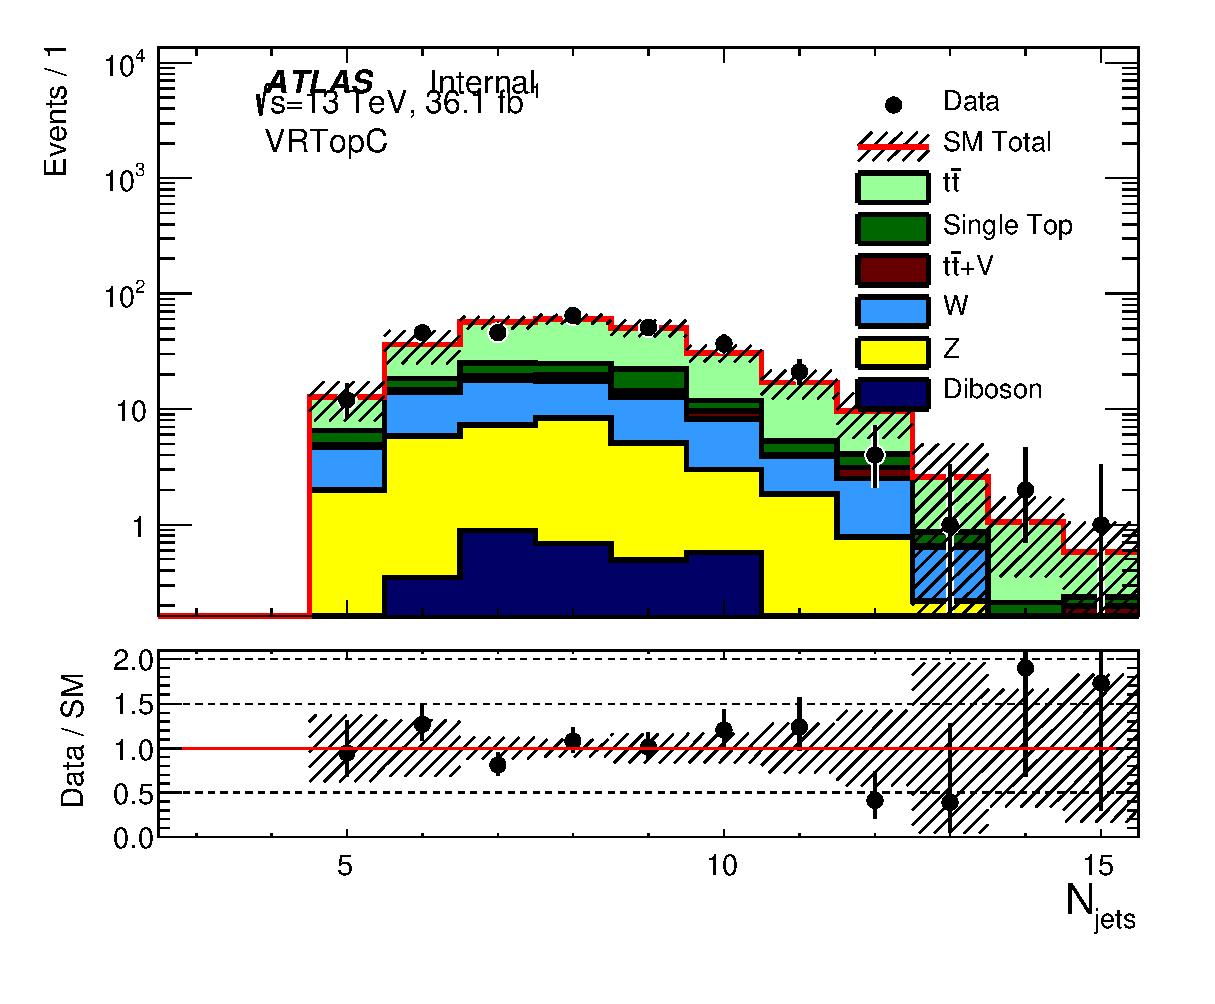
\includegraphics[width=\textwidth]{figures/plotRegion/NJets_VRTopC_log.eps}
                \caption{ }
    \end{subfigure}
    \begin{subfigure}[b]{0.40\textwidth}    
    	 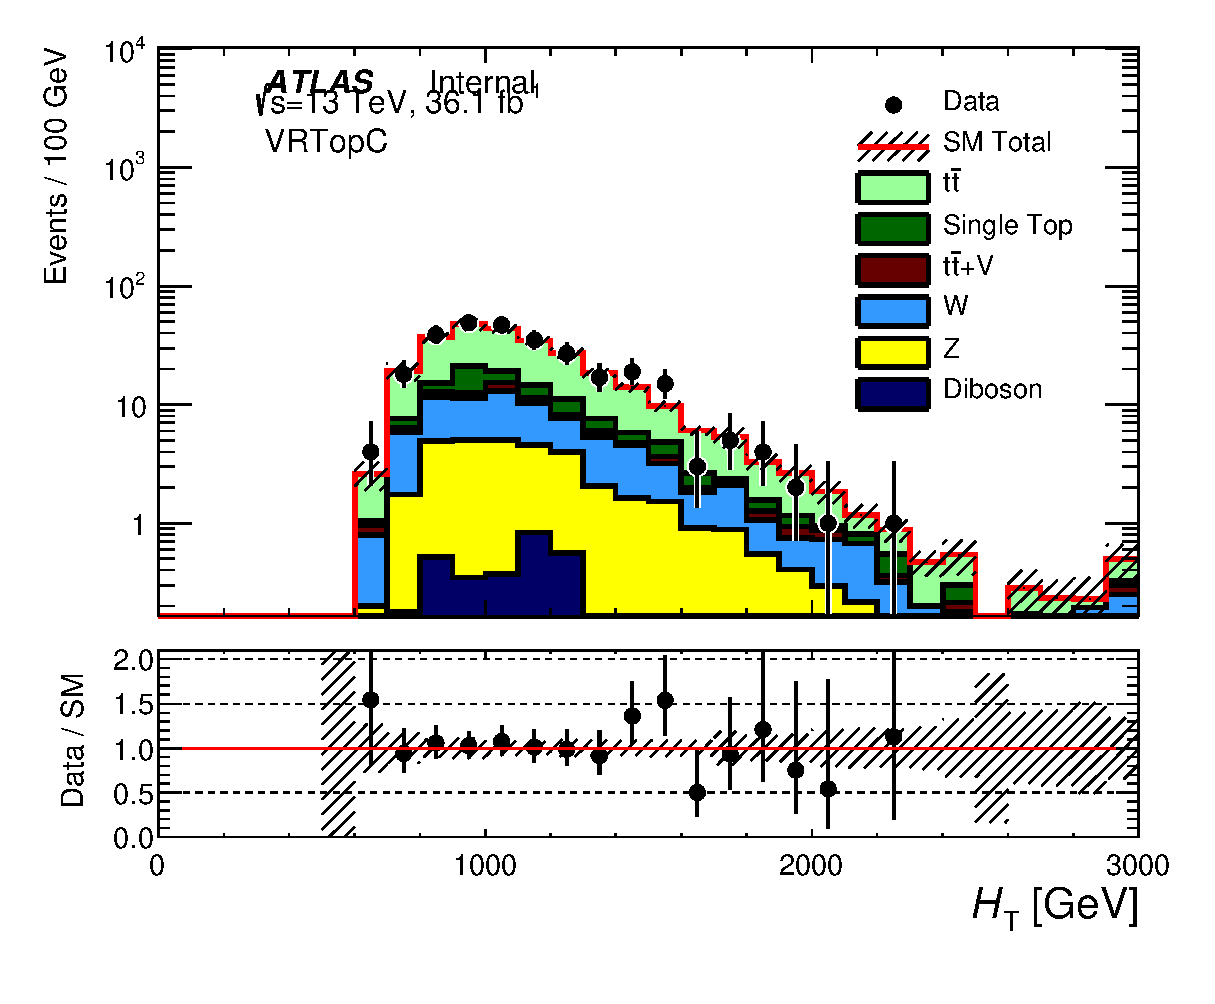
\includegraphics[width=\textwidth]{figures/plotRegion/Ht_VRTopC_log.eps}
                \caption{ }
    \end{subfigure}
    \begin{subfigure}[b]{0.40\textwidth}    
    	 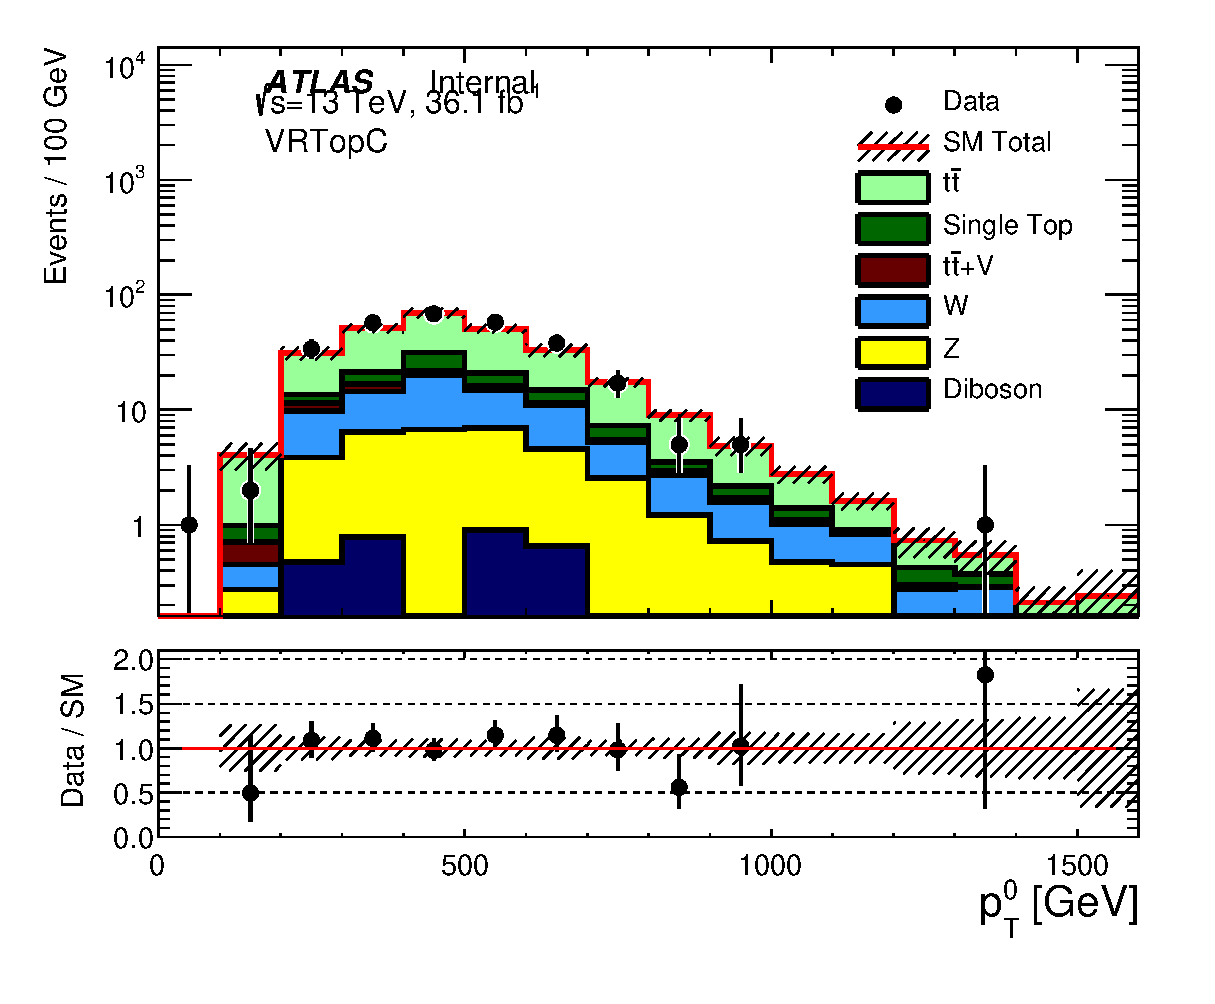
\includegraphics[width=\textwidth]{figures/plotRegion/JetPt_0__VRTopC_log.eps}
                \caption{ }
    \end{subfigure}
    \begin{subfigure}[b]{0.40\textwidth}    
    	 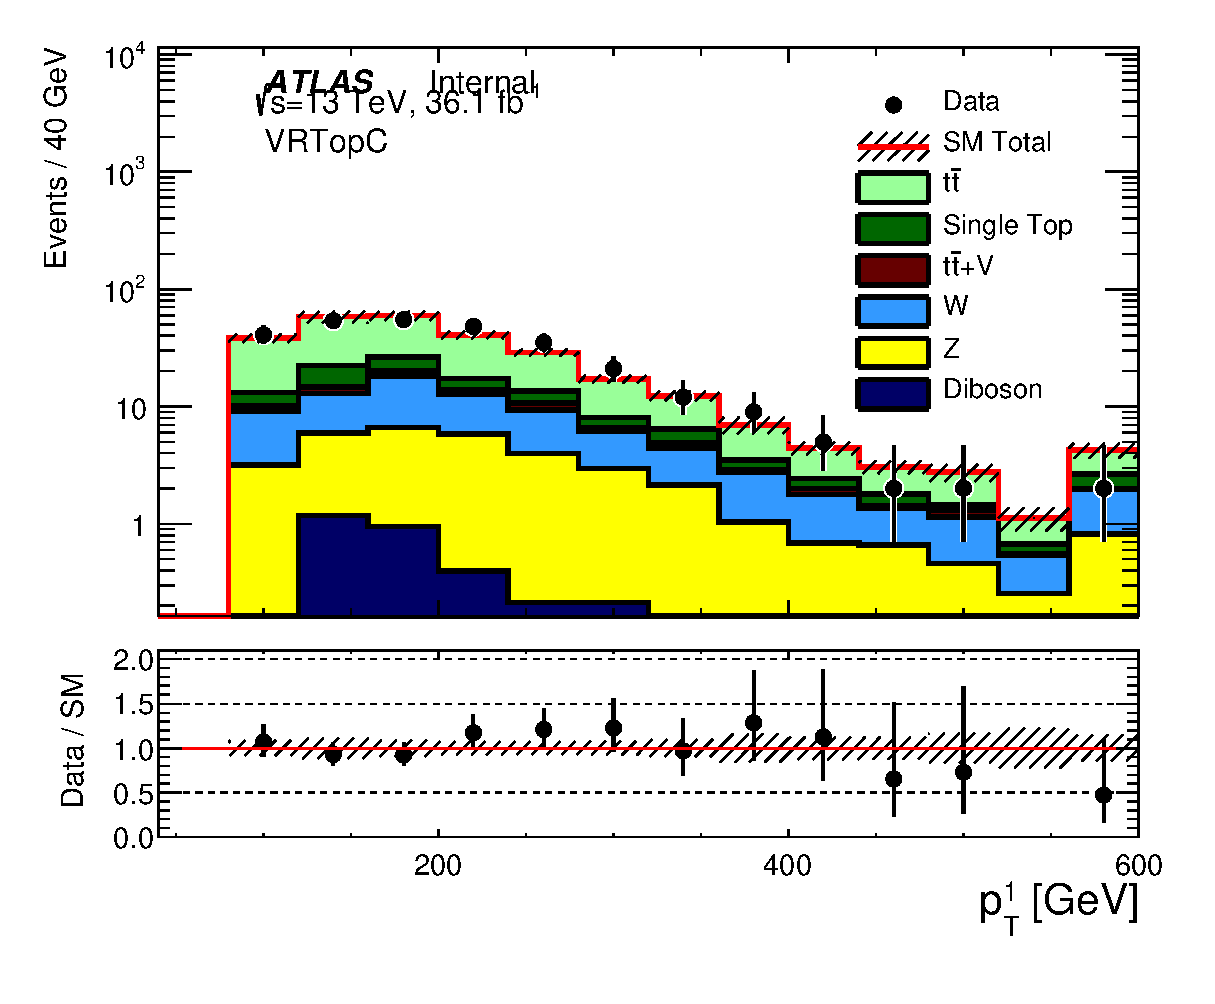
\includegraphics[width=\textwidth]{figures/plotRegion/JetPt_1__VRTopC_log.eps}
                \caption{ }
    \end{subfigure}
    \begin{subfigure}[b]{0.40\textwidth}    
    	 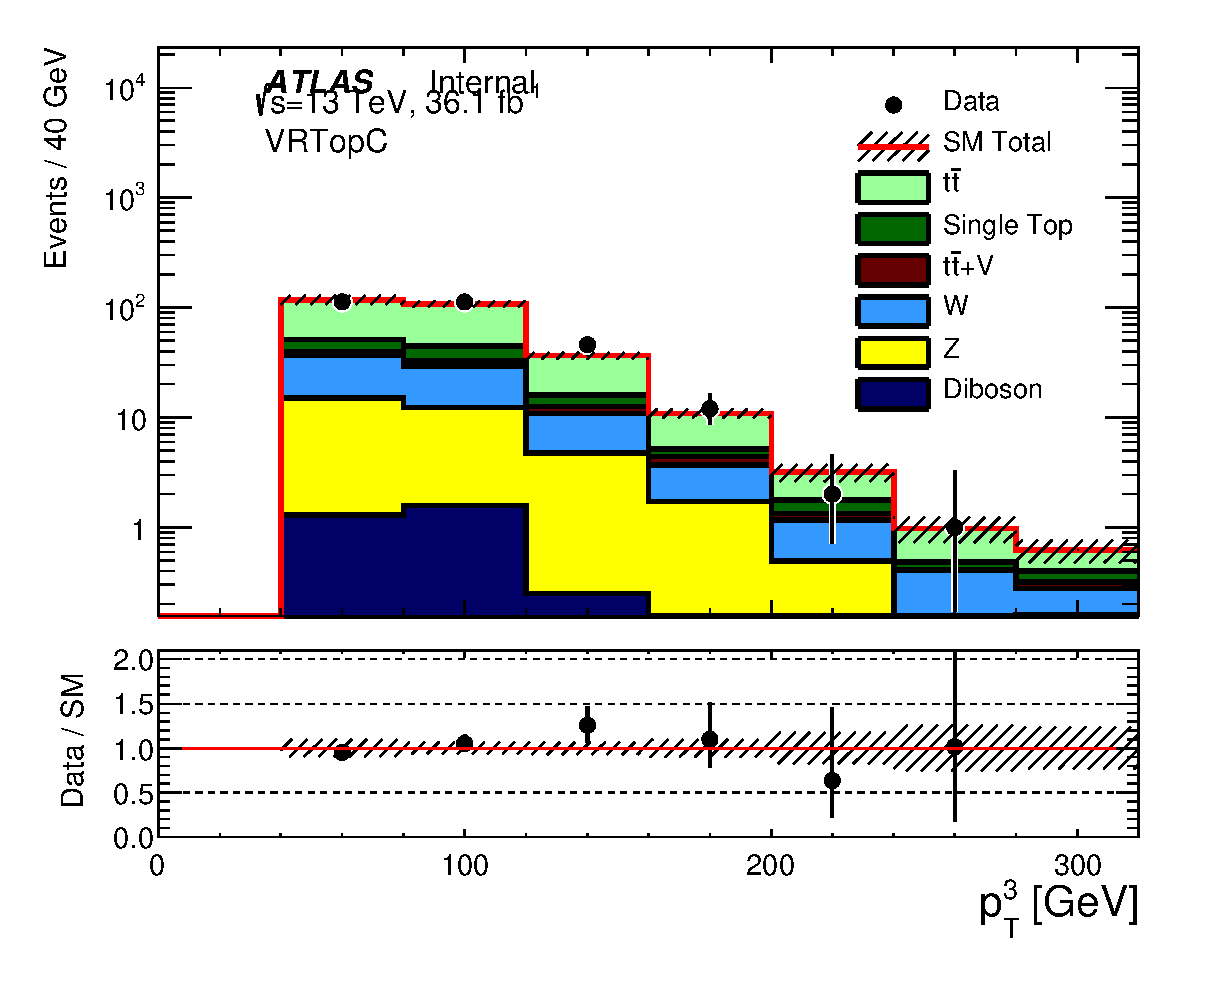
\includegraphics[width=\textwidth]{figures/plotRegion/JetPt_3__VRTopC_log.eps}
               \caption{ }
    \end{subfigure}
     \caption[Distribution of select variables in the zero-lepton $\ttbar$ validation region]{ Distribution of select variables in the zero-lepton $\ttbar$ validation region.  The kinematic variables shown include (a) $\met$ (b) number of jets (c) $\HT$ (d) $\pt$ of the highest $\pt$ jet (e) $\pt$ of the 2nd highest $\pt$ jet (f) $\pt$ of the 4th highest $\pt$ jet. }% The ratio between data and MC predictions are shown in the bottom panel.  The background rates have been normalized to control regions through a background-only fit to $\intlumi$ $\ifb$ of data.  Experimental systematic uncertainties on background predictions are depicted as the hashed bands.  }
  \label{fig:VRTopC1}
    \end{center}
\end{figure}

\pagebreak

\begin{figure}[h!]
  \centering
        \begin{subfigure}[b]{0.40\textwidth}  
	    	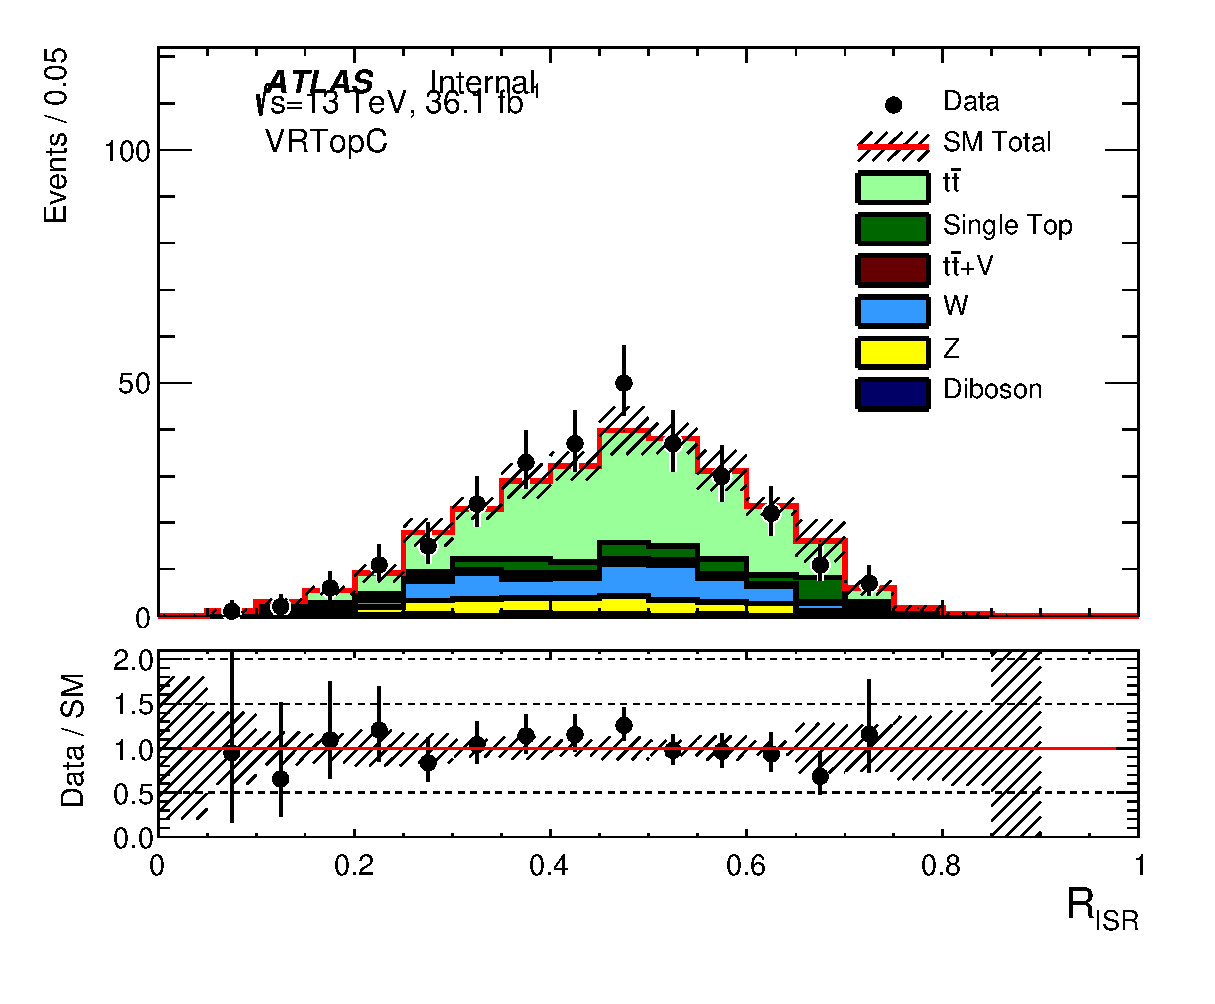
\includegraphics[width=\textwidth]{figures/ttbar/postfit/CA_RISR_VRTopC}
               \caption{ }
    \end{subfigure}
    	\begin{subfigure}[b]{0.40\textwidth}  
   		\includegraphics[width=\textwidth]{figures/ttbar/postfit/CA_pTISR_VRTopC}
               \caption{ }
    \end{subfigure}
    	\begin{subfigure}[b]{0.40\textwidth}  
    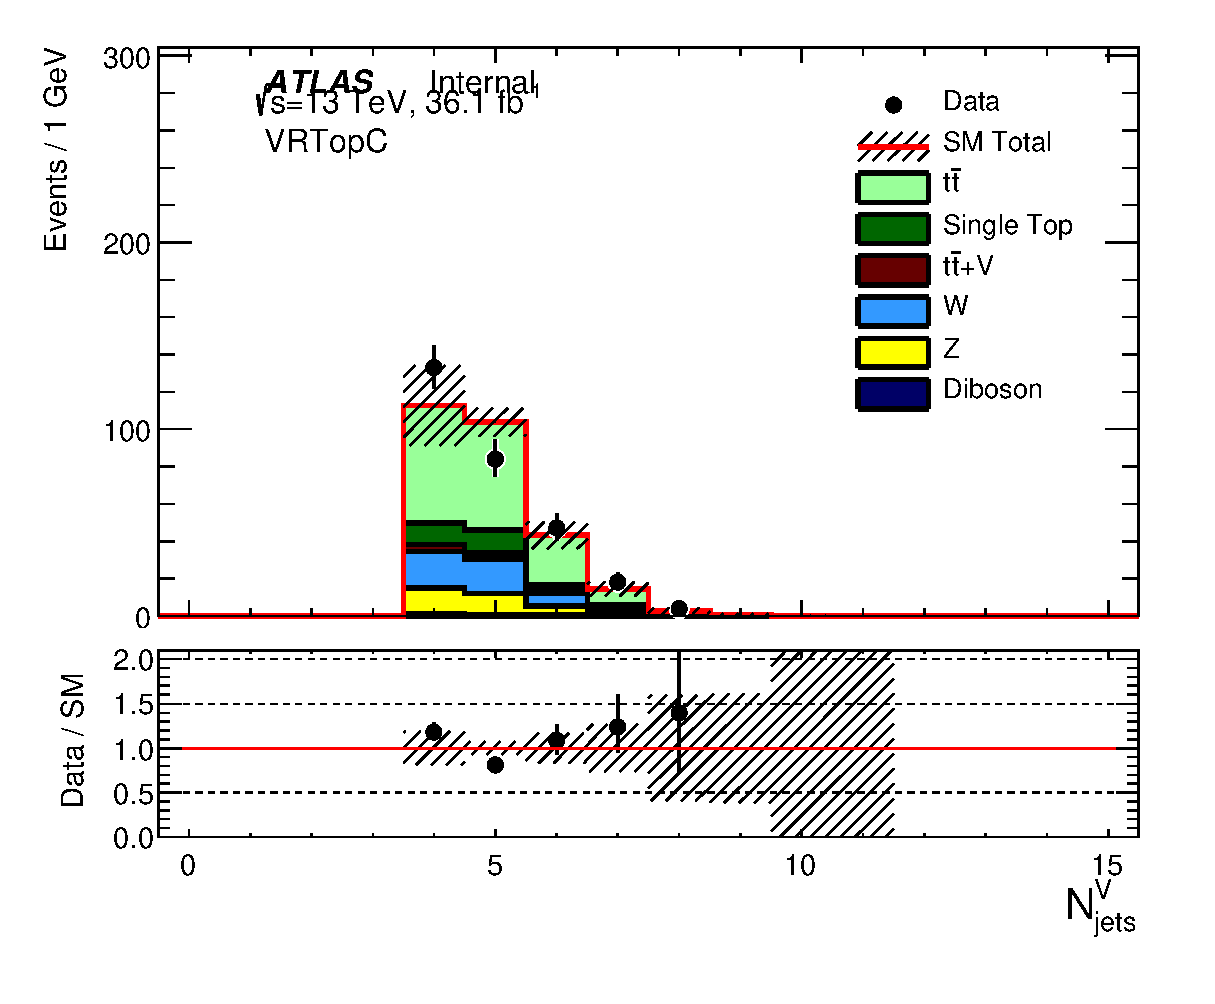
\includegraphics[width=\textwidth]{figures/ttbar/postfit/CA_NjV_VRTopC}
               \caption{ }
    \end{subfigure}
    	\begin{subfigure}[b]{0.40\textwidth}  
	    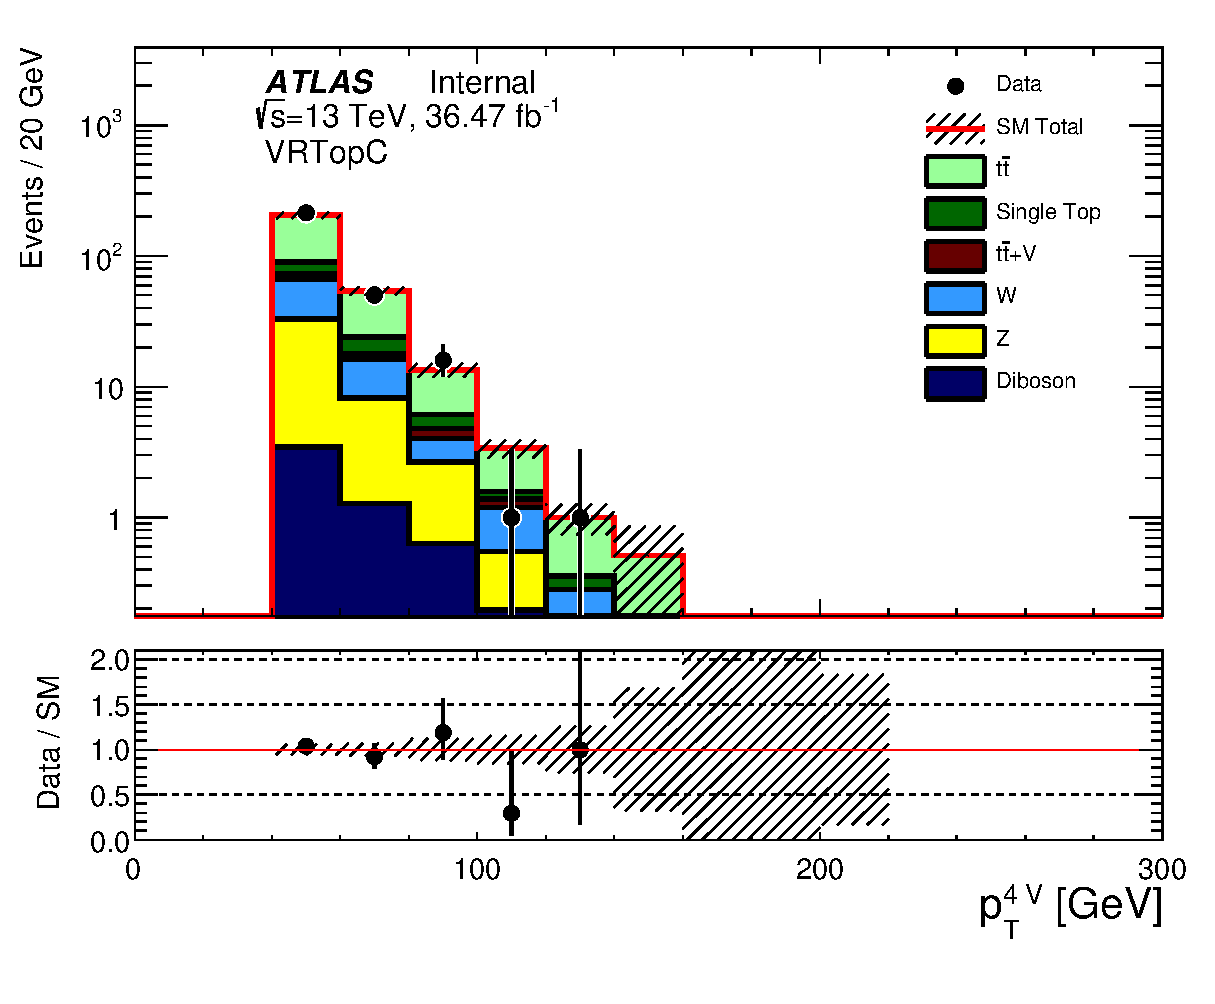
\includegraphics[width=\textwidth]{figures/ttbar/postfit/CA_pTjV4_VRTopC_log}
               \caption{ }
    \end{subfigure}
    	\begin{subfigure}[b]{0.40\textwidth}  
	    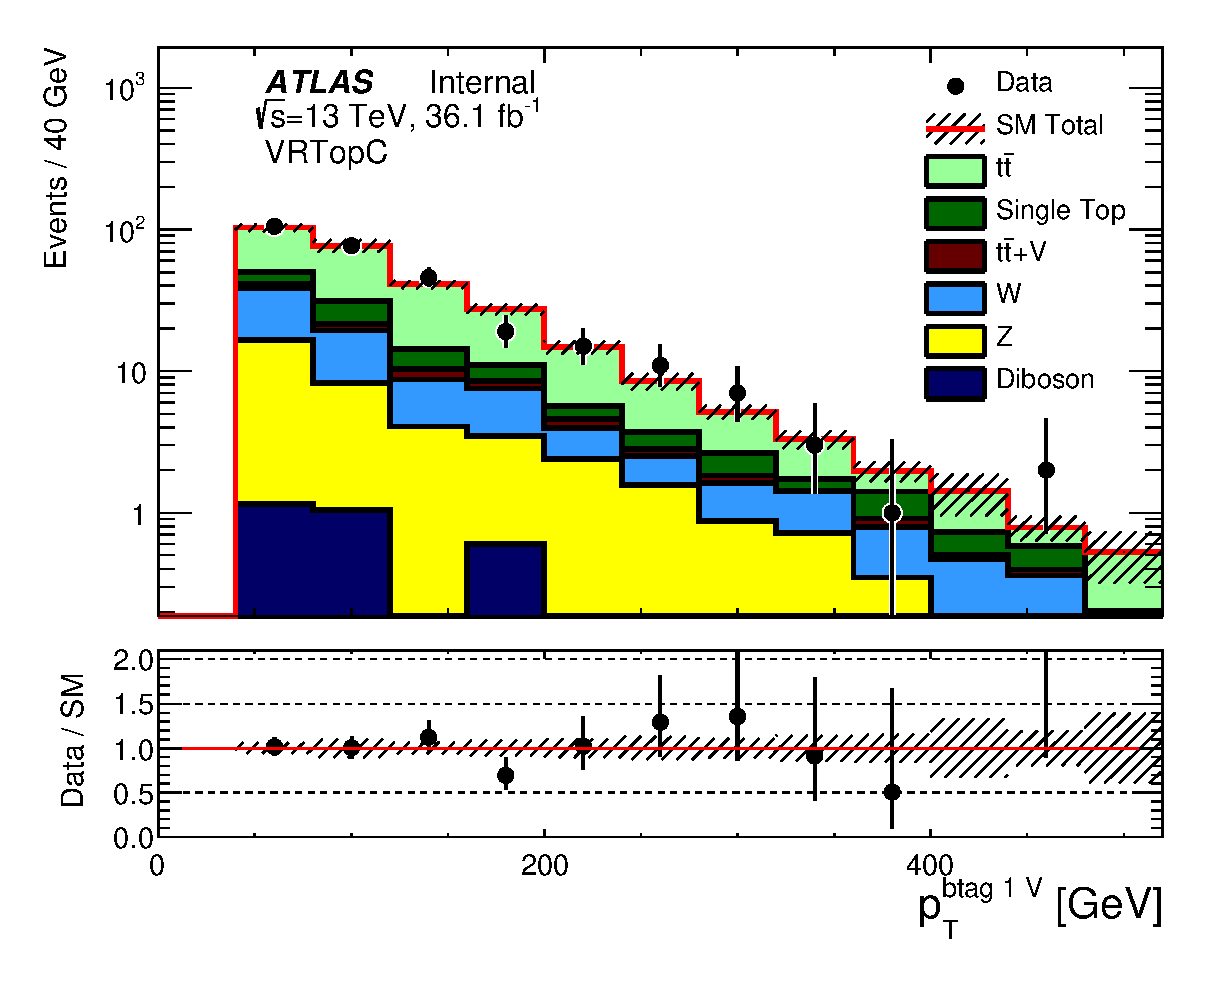
\includegraphics[width=\textwidth]{figures/ttbar/postfit/CA_pTbV1_VRTopC_log}
               \caption{ }
    \end{subfigure}
    	\begin{subfigure}[b]{0.40\textwidth}  
	    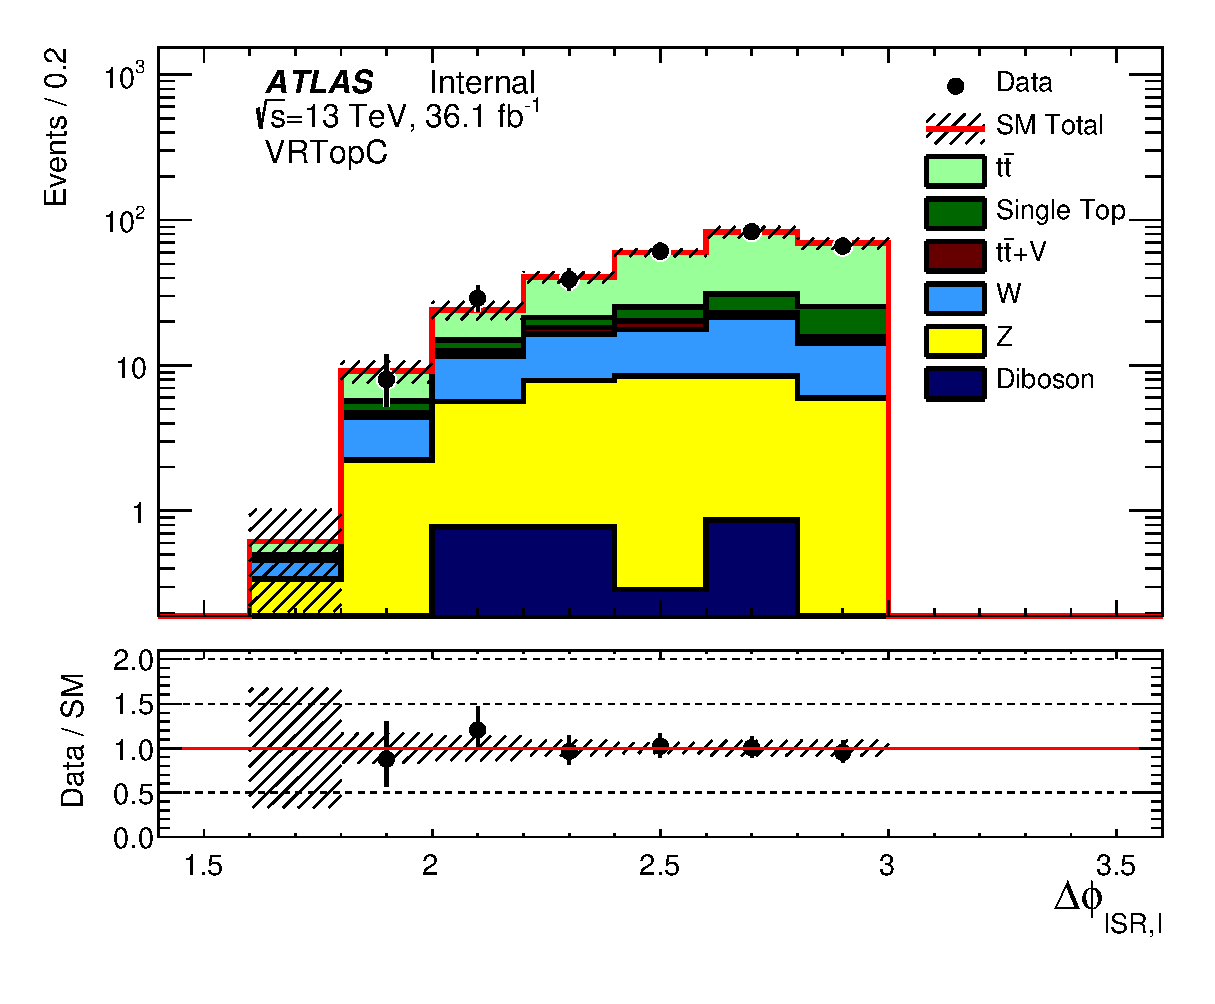
\includegraphics[width=\textwidth]{figures/ttbar/postfit/CA_dphiISRI_VRTopC_log}
               \caption{ }
    \end{subfigure}
      \caption[Distribution of select variables in the zero-lepton $\ttbar$ validation region]{Distribution of select variables in the zero-lepton $\ttbar$ validation region.  The kinematic variables shown include (a) $\RISR$ (b) $\PTISR$ (c) $\NjV$ (d) $\pTjV$ (e) $\pTbV$ (f) $\dphiISRI$. }%The ratio between data and MC predictions are shown in the bottom panel.  The background rates have been normalized to control regions through a background-only fit to $\intlumi$ $\ifb$ of data.  Experimental systematic uncertainties on background predictions are depicted as the hashed bands. }
\label{fig:ttbar0Lep1bVRISR}
\end{figure}

\indent The predicted background rate in the VRTopC agrees with data to within $1\sigma$.  This demonstrates that the control region CRTopC is an effective predictor of $\ttbar$ background rates in the validation region and the signal region.  The $\RISR$ shape is well modeled as we see no distinct trends in the data vs MC ratio in $\RISR$. \\

\indent Similar to the control region CRTopC, there is a noticeable trend in the data over MC comparison in the VRTopC $\pTISR$ distribution.  Again this is expected because the MC has a $\sim30$\% ISR/FSR uncertainties in the high ISR $\pt$ region and is a poor predictor of ISR $\pt$ rates.  \\

\indent The MC and data yields in VRTopC is given in Table \ref{table.bkgonly.VRTopC}.  The background MCs have already been normalized to their respective control regions using a background-only fit.  The validation region has the $0.707 \pm 0.050$ $\ttbar$ normalization scale factor applied to its expected $\ttbar$ MC rates.  The fact that data in VRTopC agrees with the post-fit predicted background rate is evidence that the control region CRTopC can predict the background rate in the signal region.    \\



\begin{table} [h!]
\begin{center}
\setlength{\tabcolsep}{0.0pc}
{\small
%%
\begin{tabular*}{\textwidth}{@{\extracolsep{\fill}}lr}
\noalign{\smallskip}\hline\noalign{\smallskip}
{\bf VRTop yields}           & VRTopC               \\[-0.05cm]
\noalign{\smallskip}\hline\noalign{\smallskip}
%%
Observed events          & $286$                            \\
\noalign{\smallskip}\hline\noalign{\smallskip}
%%
Fitted bkg events         & $289.20 \pm 34.10$                   \\
\noalign{\smallskip}\hline\noalign{\smallskip}
%%
        Fitted TTbar events         & $162.19 \pm 18.77$                   \\
%%
        Fitted Wjets events         & $47.37 \pm 10.17$                    \\
%%
        Fitted Zjets events         & $36.13 \pm 10.26$                   \\
%%
        Fitted TtbarV events         & $8.89 \pm 1.68$                   \\
%%
        Fitted SingleTop events         & $28.67_{-28.67}^{+30.30}$                      \\
%%
        Fitted Diboson events         & $3.00 \pm 1.86$                       \\
%%
        Fitted Multijets events         & $2.96 \pm 2.33$                      \\
%%     
 \noalign{\smallskip}\hline\noalign{\smallskip}
%%
MC exp. SM events              & $335.18 \pm 31.37$                     \\
\noalign{\smallskip}\hline\noalign{\smallskip}
%%
        MC exp. TTbar events         & $229.37 \pm 19.56$                   \\
%%
        MC exp. Wjets events         & $37.46 \pm 5.92$                      \\
%%
        MC exp. Zjets events         & $30.88 \pm 4.18$                   \\
%%
        MC exp. TtbarV events         & $6.90 \pm 1.16$                 \\
%%
        MC exp. SingleTop events         & $24.60 \pm 24.60$                     \\
%%
        MC exp. Diboson events         & $3.01 \pm 1.88$                     \\
%%
        MC exp. Multijets events         & $2.96 \pm 2.33$                 \\
%%     \\
\noalign{\smallskip}\hline\noalign{\smallskip}
Fitted \ttbar normalization scale factor & $0.707 \pm 0.050$ \\
\noalign{\smallskip}\hline\noalign{\smallskip}
\end{tabular*}
%%%
}
\end{center}
\caption[VRTopC expected background and data yields with $\intlumi$ $\ifb$ of data]{VRTopC expected background and data yields with $\intlumi$ $\ifb$ of data. MC exp. events are expected background rates directly from MC predictions.  Fitted background events correspond to the expected background rates after simultaneously fitting all control regions using a background only fit.  The backgrounds are normalized to the data in control regions and the fitted $\ttbar$ normalization scale factor derived from the fit is $0.707\pm0.050$.  The fitted normalization scale factors are then applied to the expected MC yields giving the fitted expected background rate.  The agreement between the fitted expected background yield and data in VRTopC is evidence that CRTopC is correctly measuring the amount of $\ttbar$ with high ISR $\pt$.  The quoted uncertainties include statistical and systematic uncertainties. }
\label{table.bkgonly.VRTopC}
\end{table}
%

%\indent This agreement both in magnitude and shape demonstrates two things.  One, the $\ttbar$ control region indeed does correctly measure the amount of $\ttbar$+hard ISR that exists in both signal and validation region.  Two, the subdominant background predictions also cannot by wrong by more than around 100\%.  For example we clearly would see disagreement in between data vs MC in this validation region if the MC underestimated W+jets or Z+jets background by 100\%.  Both of these facts give us confidence that the background prediction in the signal region is correct. \\